\documentclass[master,oneside,euler,openright,macfonts]{ustcthesis}
% 默认twoside 双面打印
% 将master修改为bachelor, doctor or master
% 要使用adobe字体,添加adobefonts选项
% 要使用Mac系统的字体,添加macfonts选项
% 使用euler数学字体,如不愿使用,去掉euler
% 使用外文写作,请添加notchinese

% 设置图形文件的搜索路径
\graphicspath{{figures/}}

%仅用于本示例文档中显示特殊字符串
\usepackage{xltxtra}
\usepackage{listings}
\usepackage{color}
\usepackage{hyperref}

\definecolor{dkgreen}{rgb}{0,0.6,0}
\definecolor{gray}{rgb}{0.5,0.5,0.5}
\definecolor{mauve}{rgb}{0.58,0,0.82}

\lstset{frame=tb,
  language=Java,
  aboveskip=3mm,
  belowskip=3mm,
  showstringspaces=false,
  columns=flexible,
  basicstyle={\small\ttfamily},
  numbers=none,
  numberstyle=\tiny\color{gray},
  keywordstyle=\color{blue},
  commentstyle=\color{dkgreen},
  stringstyle=\color{mauve},
  breaklines=true,
  breakatwhitespace=true,
  tabsize=3
}

\colorlet{punct}{red!60!black}
\definecolor{background}{HTML}{EEEEEE}
\definecolor{delim}{RGB}{20,105,176}
\colorlet{numb}{magenta!60!black}

\lstdefinelanguage{json}{
    basicstyle=\normalfont\ttfamily,
    numbers=left,
    numberstyle=\scriptsize,
    stepnumber=1,
    numbersep=8pt,
    showstringspaces=false,
    breaklines=true,
    frame=lines,
    backgroundcolor=\color{background},
    literate=
     *{0}{{{\color{numb}0}}}{1}
      {1}{{{\color{numb}1}}}{1}
      {2}{{{\color{numb}2}}}{1}
      {3}{{{\color{numb}3}}}{1}
      {4}{{{\color{numb}4}}}{1}
      {5}{{{\color{numb}5}}}{1}
      {6}{{{\color{numb}6}}}{1}
      {7}{{{\color{numb}7}}}{1}
      {8}{{{\color{numb}8}}}{1}
      {9}{{{\color{numb}9}}}{1}
      {:}{{{\color{punct}{:}}}}{1}
      {,}{{{\color{punct}{,}}}}{1}
      {\{}{{{\color{delim}{\{}}}}{1}
      {\}}{{{\color{delim}{\}}}}}{1}
      {[}{{{\color{delim}{[}}}}{1}
      {]}{{{\color{delim}{]}}}}{1},
}

%%%%%%%%%%%%%%%%%%%%%%%%%%%%%%
%% 封面部分
%%%%%%%%%%%%%%%%%%%%%%%%%%%%%%

  % 中文封面内容
  \title{基于手机主题推荐系统的用户画像模型}%一般情况下扉页和封皮、书脊共用一个标题文本,可以不用定义\spinetitle(仅硕博有用), \covertitle(本硕博均有用)和\encovertitle(仅本科有用)。特殊情况见下。
  %\spinetitle{\small{中国科学技术大学本硕博毕业论文模板示例文档\raisebox{-3pt}{(Beta)}}}
  %特殊情况1:本例中\title命令里含有换行控制字符,这会导致制作书脊的时候出现错误,例如如果你注释掉\spinetitle{...}这一行就会报错。这时需要定义一个不含换行等命令的\spinetitle,这并不表示\spinetitle里不能有任何命令——只能使用有限的命令。
  %特殊情况2:本例中标题过长,所以需要缩小书脊标题的字号。
  %特殊情况3:本例中中英文混排,由于tex竖排的原理限制,中英文基线不重合,所以需要人工调整英文的基线。具体调整量根据不同字体有所不同。
  %\covertitle{中国科学技术大学本硕博毕业\\论文模板示例文档(Beta)}
  %\covertitle{中文题目第一行\\中文题目第二行}
  %不要在此调整封皮字体大小! Do not set Cover Page font size here!
  %特殊情况4:本例中\title中含有多个换行,导致标题超过了两行。根据制本厂规定,封皮标题不能超过两行。因此需要定义封皮使用的标题\covertitle. 如果你注释掉这一行,就会发现封皮不符合规定。
 % \encovertitle{USTC Thesis Template for Bachelor, Master and Doctor User's Guide(Beta)}
  %\encovertitle{English Title Line 1\\English Title Line 2\\English Title Line 3}
  %不要在此调整封皮字体大小! Do not set Cover Page font size here!
  %特殊情况5:仅本科生有用。本科封皮中有英文标题,不超过三行。与上类似。

  \author{胡磊}
  \depart{软件学院}%系别,硕博请用系代号,本科请用全称如
  %\depart{数理化和信息工程系}
  \major{信息安全专业}%专业,硕博请用全称,本科不需要
  \advisor{周武旸\ 教授}
  \coadvisor{张四海\ 博士}%第二导师,没有请注释掉
  \studentid{SA13226110}%For bachelor only
  \submitdate{二〇一六年四月}

  % 英文封面内容
  \entitle{The User Profile Based on Phone Theme Recommendation System}
  \enauthor{Lei Hu}
  \enmajor{Information Security}
  \enadvisor{Prof. Wuyang Zhou}
  \encoadvisor{Dr. Sihai Zhang}%另外一个导师
  \ensubmitdate{April 21th, 2016}
  
%%%%%%%%%%%%%%%%%%%%%%%%%%%%%%%%%%%%%%%%%%%%%%%%%%%%%%%%%%%%%%%%%%%%%

\begin{document}

  % 封面
  \maketitle

%特别注意,以下述顺序为准,在对应部分添加文档部件,切勿颠倒顺序:
%本科论文的文档部件顺序是:
%    frontmatter:致谢、目录、中文摘要、英文摘要、
%    mainmatter: 正文章节
%    backmatter: 参考文献或资料注释、附录
%硕博论文的文档部件顺序是:
%    frontmatter:中文摘要、英文摘要、目录、符号说明
%    mainmatter: 正文章节
%    backmatter: 参考文献、附录、致谢、发表论文
%%%%%%%%%%%%%%%%%%%%%%%%%%%%%%
%% 前言部分
%%%%%%%%%%%%%%%%%%%%%%%%%%%%%%
\frontmatter
\makeatletter
\ifustc@bachelor
	%%%%%%%%%%%%%%%%%
	%本科论文修改这里
	%%%%%%%%%%%%%%%%%
	% 致谢
	
\begin{thanks}

人生就是一个关于成长的漫长故事。而在中科大求学作为本人人生体验的一部分,亦是这样的一段故事。在此的俩年半,俯仰之间,科大的“问道”、“学术”于此,让我经历了这样的三段成长:学于师友,安于爱好,观于内心。

“古之学者必有师,师者,所以传道、授业、解惑也”。师友的教诲不可能一直跟着自己,可是他们治学态度却融入了我的人生观。授课的华保健老师的严谨、郭燕老师的认真、丁菁老师的直率、席菁老师的踏实都曾触动我,并给予我前进方向上的指引。

本论文内容为数据挖掘在电商行业的工程实现,因此有一段真实的、贴近数据挖掘领域的实习经历尤为重要。感谢我在苏州国云数据公司实习的 CEO 马晓东学长,让我有机会一窥大数据行业的内幕;感谢我在小米实习的导师方流博士,感谢我在滴滴出行工作的机器学习研究院李佩博士,让我成为大数据挖掘工程师的梦想又更近了一步;感谢我的导师周武旸教授和张四海教授,指导我完成论文。
向师友和书籍学习,是从外界汲取;只有回归到自己的内心和思绪才能沉淀.在每个夜幕深沉或是晨曦初露的时刻里,感受自己情绪的流动,反思自己的取舍得失,然后才有了融于师友和书籍时的奋进。这样的三段成长,如今已是一体,不断地相互印证与反馈!

“逝者如斯夫,不舍昼夜”。成长亦复如是,不断的和昨日的自己告别。但是,一路有你,真好!相会是缘,同行是乐,共事是福!

\vskip 18pt

\begin{flushright}

~~~~\ustc@author~~~~

\today

\end{flushright}

\end{thanks}

	
	%目录部分
	%目录
	\tableofcontents
	%默认表格、插图、算法索引名称分别为“表格索引”、“插图索引”和“算法索引”
	%如果需要自行修改lot,lof,loa的名称,请定义
	%\ustclotname{...}
	%\ustclofname{...}
	%\ustcloaname{...}

	% 表格索引
	\ustclot
	% 插图索引
	\ustclof
	%算法索引 
	%如果需要使用算法环境并列出算法索引,请加入补充宏包。
	\ustcloa
	
	% 摘要
	 %\begin{cnabstract}
本文是中国科学技术大学本硕博毕业论文模板示例文件。本模板由ywg@USTC创建,适用于撰写学士、硕士和博士学位论文,本模板由原来的本科模板和硕博模板整合优化而来。本示例文件除了介绍本模板的基础用法外,本文还是一个简要的学位论文写作指南。

\keywords{中国科学技术大学\enskip 学位论文\enskip \LaTeX{}~通用模板\enskip 学士\enskip 硕士\enskip 博士}
\end{cnabstract}

\begin{enabstract}
Because of the dynamic evolution and propagation of the Internet and the popularization of social networks, huge amounts of information about the users's behaviour are accessible to commercial internet companies. Most companies can be easily approaching OOS(open source software) such as hadoop to analyse and interpreting users's behaviour data-set,which just several years ago was not available or inaccessible. Also because of the evolution and popularization of the Internet and the vast amount of data stored, it has become desirable to moderate and select the content that is being displayed to the user,Mechanisms presenting goods on application try to present content that can interest the user based on his previous queries or browsing history. commercial internet companies such as e.g. Xiaomi filter the phone theme application visiting information and show only phone themes that the user potentially be interested in, trying to sell additional goods by recommender products based on user previous purchase behaviours.

Based on my working experience on Xiaomi as internship, The biggest challenge of recommender systems in commercial internet companies is: How to optimize a recommender system in accordance with the true business objective. for commercial internet company like Xiaomi the fitness recommender system is something that mix the social part, the long-tail, the cold-start and many other factors to finally aproximate what the user really wants. It's really a fascinating and complex working. 

The aim of this paper is analyse the long tail feature and cold start feature of a android phone theme recommender system with the help of user profiles and user interests exploration. In order to build the user profile, Information Retrieval (IR) and Data Mining (DM) techniques such as content-based Collaborative Recommendation and text pre-processing methods have been used; In order to approaching discovery and recommendation in long tail, user interests exploration has been refered. Because of the subjective nature of such a solution, verification process such as A/B test is also introduced.

\enkeywords{recommender systems, long tail, cold start, user profile, user interests exploration}
\end{enabstract}
%此文件中含有中英文摘要
\else
	%%%%%%%%%%%%%%%%%
	%硕博论文修改这里
	%%%%%%%%%%%%%%%%%
	% 摘要
	 \begin{cnabstract}
信息爆炸使得用户很难有效的从海量的数据中快速获取自己需要的信息,推荐系统凭借精准定位和"千人千面"的个性化服务受到互联网企业的青睐和研究者的重视。本论文讨论了如何构建一个基于手机主题推荐系统的用户画像模块和用户兴趣探索模块。

传统的个性化推荐系统面临着诸多挑战,其中最根本的问题是如何根据企业的商业目标和业务特点来优化推荐系统,具体到手机主题行业,推荐系统需要解决社交化、长尾性、冷启动、动态推荐等一系列综合问题。由此,笔者提出并实现了一种适用于手机主题个性化推荐系统的用户画像模型,本文的主要工作和贡献有:
\begin{itemize}
	\item 实现了推荐系统的用户画像模块。利用信息检索(Information Retrieval)技术从用户注册信息获取到用户的人口属性、职业、地理位置、性别等信息并标签化,不同标签的来源,标签的本身,以及标签与用户之间的共现关系决定着这个标签的初始权重,然后根据用户行为构建相应的AB测试产出标签的实际权重,权重越高则认为该标签对用户影响越大。AB测试显示推荐系统利用用户画像标签进行推荐能显著提升诸如点击转换率等重要指标。
	\item 实现了推荐系统的用户兴趣探索模块。用户兴趣探索通过特征提取技术和用户满意度量化算法,定期更新用户兴趣标签和标签对应的权重。首先,利用用户兴趣特征向量和商品特征向量计算出用户-商品的相关分数。然后,利用用户行为(购买、评分、点赞、划屏频率等)量化用户满意度。一次成功的用户兴趣标签探索,首先应该有很低的相关分数和很高的满意度,其次兴趣标签应该是一个小众兴趣标签。用户兴趣探索能够实时更新用户的兴趣标签,帮助推荐系统持续满足用户的不断变化的需求。
	\item 利用时间因子衰减模型融合用户的长期兴趣和短期兴趣:用户画像针对的是用户的静态信息,代表了用户的长期兴趣,用户兴趣探索针对的是用户的动态信息,代表了用户的短期兴趣,衰减模型法的本质是利用自然遗忘规律对用户的兴趣进行衰减。
\end{itemize}

\keywords{推荐系统\enskip 长尾效应\enskip 动态兴趣\enskip 用户画像建模\enskip 用户兴趣探索\enskip}
\end{cnabstract}

\begin{enabstract}
Information explosion in the new age let it's hard for users to get valuable infomation from the vast amounts of data, so the recommended system begin to go to the middle of the stage because it's precise forecast and Personalized service. So we here to discuss how to modeling users profile model and users interested exploration model for a android phone theme application recommended system.

There are so many weekness of the traditional recommended system, the most import one is how to sell more products, specific for android phone application, the recommended system need to solve Socializing problem, cool start problem, dynamic recommend based on timeline and so on. So the author proposed and implemented users profile model and users interested exploration model which include: 
\begin{itemize}
	\item Realized the use profile model of recommended system, we use information retrieval technology to get use basic information like occupation, location, gender from user registration information, different tag has different weight depending on the way they got, the path of they transfer and the relation between use and tags, the more weight of tag the high of credibility the tag has. AB test show that recommended system can improve click conversion rate rapidly.
	\item Realized the users interested exploration model of recommended system, which using feature extraction technology and user satisfaction scoring algorithm, we maintain a dynamic interesting tags vector space for all user. first, we can get user-item-scores by product users interesting vector metric and items feature metric. Then get the users satisfaction based on users history actions like buying, rateing, clicking and so on. one successful exploration means it has low user-item-relation-scores and high user satisfaction, and the tag also is minority. Experiments show that with the users interested exploration model, the recommended system has more long-tail effect.
	\item Sucessfully put user long term interesting and short term interesting into one model using linear decay algorithm, users profile model contains static infomation of users, users interested exploration model contains dynamic infomation of users interesting, this papar come up with the strategy to balance the static infomation and the dynamic infomation.
\end{itemize}
\enkeywords{recommend system, long-tail, dynamic, user profile, user interest explore}
\end{enabstract}
%此文件中含有中英文摘要
	% 目录
	\tableofcontents
	%默认表格、插图、算法索引名称分别为“表格索引”、“插图索引”和“算法索引”
	%如果需要自行修改lot,lof,loa的名称,请定义
	%\ustclotname{...}
	%\ustclofname{...}
	%\ustcloaname{...}

	% 表格索引
	\ustclot
	% 插图索引
	\ustclof
	%算法索引 
	%如果需要使用算法环境并列出算法索引,请加入补充宏包。
	%\ustcloa
	
	%符号说明,需要加入补充包
	 %\begin{denotation}

\item[] 
\end{denotation}
%不是必需的,如果不想列出请注释掉
\fi
\makeatother

%%%%%%%%%%%%%%%%%%%%%%%%%%%%%%
%% 正文部分
%%%%%%%%%%%%%%%%%%%%%%%%%%%%%%
\mainmatter

   
\chapter{绪论}
\label{chap:introduction}
\section{研究背景与意义}
	互联网自二十世纪九十年代从诞生、发展,到现在已经演化为人类社会的必需品。随着互联网的发展,用户的信息检索模式也发生了翻天覆地的变化,早期用户可以毫不费力的直接记住寥寥无几的网站、网址,轻松实现上网需求;随着网站呈指数的发展,网址数量大大超出人脑记录的容量,于是Yahoo!公司首次提出并实现了分类目录系统的概念,其本质还是通过人工将网站分门别类,因此其创新还是属于量变,没有达到质变。随着网站进入到爆发式增长,人工实现分类目录法变得越来越不现实了,于是产生Google为代表的搜索引擎,搜索引擎实现了互联网的质变,通过程序自动化的实现了检索网站、爬取内容、存储数据,实现了亿万级的数据积累,只有基于如此庞大的信息,才能为哪怕是最普通的用户提供及时、准确、快速信息获取服务,人类社会一定程度上填平了所谓的“信息鸿沟”。但是,后互联网时代又是个性化时代\citep{Personalization1,Personalization2,Personalization3,Personalization4,Personalization5,Personalization6,Personalization7,Personalization8,Personalization9},需要一种系统精确刻画每个用户的兴趣爱好并能不动声色的在主页上表现出来,我们把这种提供个性化服务的系统系统统称为推荐系统。推荐系统是一种比搜索引擎更人性化、个性化的系统服务,不需要用户主动提供关键词,因此它能满足用户的更多的潜在需求,尤其当用户自己都无法精准描述自身需求的时候\citep{recmd-system}。第一代推荐系统以亚马逊为代表,作为一个电子商品平台,一方面有数以万计的商品需要被用户了解、熟悉和购买,另一方面有数以亿计的用户无法找到称心如意的商品。推荐系统通过构建用户和商品之间的桥梁,每年为亚马逊贡献近三十个百分点的创收!由此可见推荐系统能帮助用户快速发现有用的商品信息,具体来讲,首先推荐系统通过分析用户的历史行为每个用户进行独一无二的画像建模\citep{demo-data},目的有俩个:1,熟悉每个用户和他们的潜在需求;2,把拥有相同品味的用户归为一类群体,这样一来所有人的需求总和就可能是其中一个人的潜在需求,方便企业卖出更多的商品。随着用户终端设备的普及,出现了诸如淘宝、美团、滴滴、今日头条等互联网平台,几乎包办了人们衣食住行的方方面面,人们因为可选择性太多而出现了“选择性困难”的症状,这其实就是信息过载时代的具体表现形式。也就是说,在这个数据爆炸时代,无论是作为信息消费者的普通用户,还是作为信息生产者的提供商,都面临着日益严峻的挑战,现代人每天面临着从各种不必要的数据中找到有用的商品,其实是在浪费生命。每一个有追求、有理想的现代人,真的需要好好的设计人生,以一种精要的方式摒弃不必要之事,而这也是林语堂先生所说的生之智慧。笔者曾有过这样的一种购物体经历:笔者在淘宝商城购买一台笔记本电脑,花费了一上午的时间才浏览、比较完所有的 thinkpad 品牌商家店面,如\autoref{fig:hl_taobao}。
	\begin{figure}
		\centering
		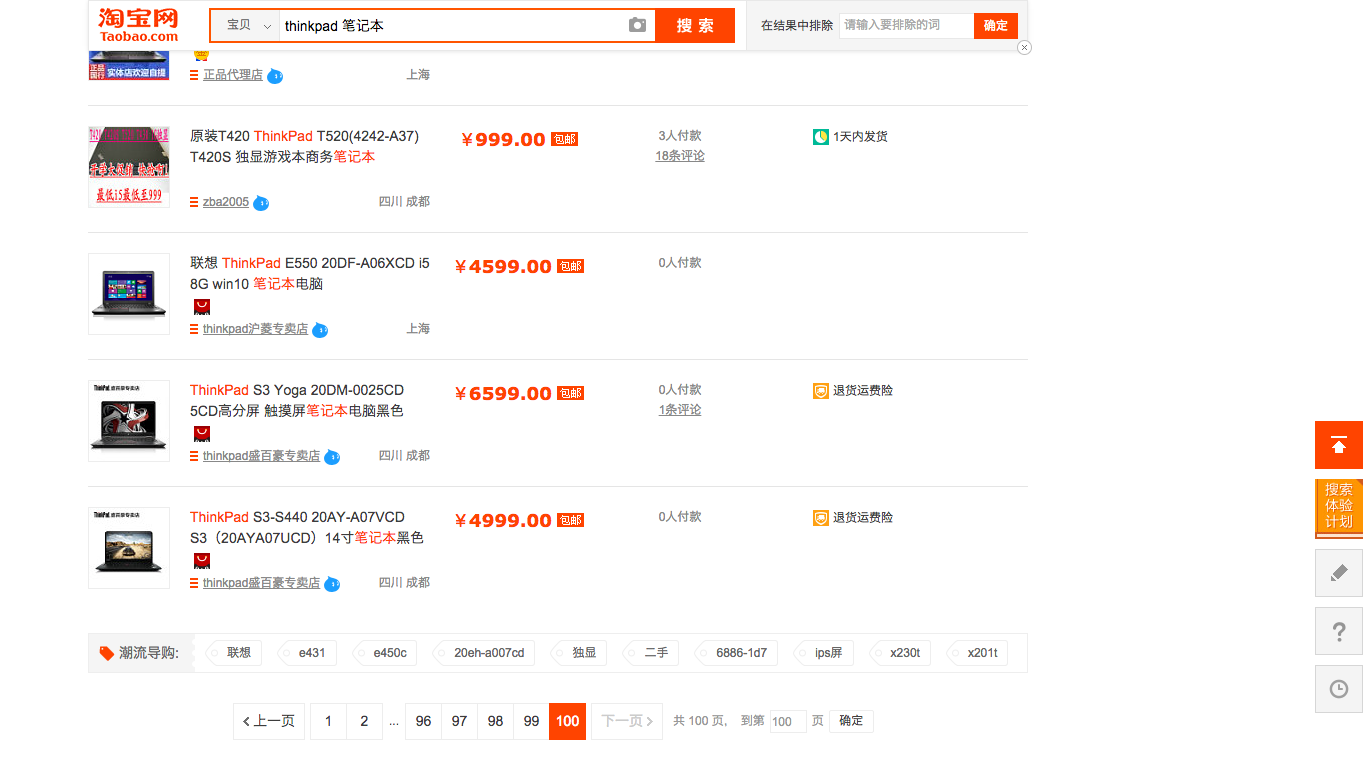
\includegraphics[width=0.9\textwidth]{hl_taobao}
		\figcaption{淘宝购物搜索图}
		\label{fig:hl_taobao}
	\end{figure}
	其实,作为互联网电子商家的翘楚---淘宝,一直在思考如何让自己平台下的优秀商品不埋没在大数据洪流中,因此,淘宝技术团队一直把个性化推荐系统视为解决用户-商品合理匹配的终极杀手锏。对于一个电商平台,原则上商品肯定是多多益善,但对于一个个性化推荐系统,则遵守更少,但更好的原则,推荐系统代表了一种自律的、精要的生活方式,据笔者所知,已经有很多互联网企业已经或者正在开发符合其企业文化的推荐系统,如笔者曾供职过的小米、今日头条和滴滴出行,其中小米的广告部门很早就利用推荐算法实现旗下各个业务线的只能广告投放,而今日头条利用推荐系统每日为用户定时推荐文章,滴滴出行则利用推荐系统为每个乘客和网约车做定向匹配。对于传统的推荐系统,首先,需要积累足够多的商品信息,因为只有尽可能的在基于所有的商品大局观上,才有可能得出比较正确的商品推荐候选集合;其次,需要尽可能积累用户的行为数据,因为这些数据将会是推荐统计假设检验的唯一数据标准,统计学之所以常让人意外,就是因为人们常常只能得到一部分的样本,而这些样本只是包含了部分而不是全部数据的信息,就有扭曲事情本质的趋势,因此,精度是推荐系统最重要的指标之一,后文会详细介绍如果通过用户画像和用户兴趣\citep{user-interests-explore,user-interests-explore1,user-interests-explore2,user-interests-explore3,user-interests-explore4}提升推荐系统的精度;最后就是甄别,哪些商品对哪些用户有着非同寻常的吸引力,其实对于一个用户来讲,平台上存在的绝大多数商品,包括数据、资源和他人观点,都没有什么价值,只有少数商品效果非凡,影响巨大,推荐系统的核心就是算法,通过算法甄别无意义的多数,只留下有意义的少数。总之,通过算法分析用户兴趣,分析商品特性,为每一个人,对所有商品打分、排序、取topN,找到用户感兴趣的商品,然后得出推荐结果,给用户他们想要的。

	但是,传统的推荐系统也有一些问题,典型的有数据稀疏问题、新用户问题、马太效应、实时推荐问题和用户兴趣变动问题。数据稀疏问题的本质就是商品信息数据过于膨胀,即使是骨灰级用户也没办法穷尽百分之一的商品,因此大多数的用户-商品相关值都是零,这不利于推荐系统做出正确的推荐结果;新用户问题又叫冷启动问题,指一个用户刚刚注册登录,推荐系统没有与此人相关的信息,于是就没有方法做出推荐;马太效应是指越热门的商品越有被推荐的趋势,这种情况其实不是一件好事,因为:1,商品营收不平衡会增加平台的风险性,如果平台大多数营收的贡献来自于若干类商品,一旦这类商品发生问题,平台也会有问题;2,根据2/8原则,冷门商品虽然营收少,但它们的基数大,潜力无限;实时推荐问题是指用户从浏览到购买这段时间一般很短,而推荐系统需要打时间差,在用户购买之前就做出推荐,但这是很难实现的,因为对所有商品打分、排序、取 topN,最后找到用户感兴趣的商品,在工程上是需要一些时间的;用户兴趣变动问题是指用户兴趣是一个动态的过程,有可能随着季节周期性变动,有可能随着年龄发散性变化,推荐系统需要及时收集数据,保持对用户兴趣的最优拟合。

	基于这些问题的存在,笔者基于推荐系统实现了用户画像模块和用户兴趣探索模块,帮助推荐系统做出更好的推荐结果。用户画像模块其实就是回归了问题的本质:以人为本,用数据说话。通过分析、收集所有与用户有关的数据,为每个用户建立、维护一个独一无二的用户画像,用户画像的最大优点在于它能主动收集用户的基本人口数据、长期兴趣和短期兴趣,而且用户画像中的信息是动态更新的,也就是说随着时间的推移,用户的兴趣在逐渐改变,用户画像里的兴趣标签也会随之改变,最大程度上保证了用户兴趣的连续性和变化性;用户兴趣探索模块包括三个原则:1,用户和潜在感兴趣商品的关联度很低,这保证了探索的商品都是用户从前没有看见过的;2,用户满意度很高,这是通过利用用户行为,包括点击次数、滑屏次数、滑屏频率、滑屏时长、点赞、分享等行为,量化了用户的满意度;3,潜在商品的标签是小众的、冷门的标签,因为热门商品是没必要也不需要做探索的。

\section{推荐系统的简介}
推荐系统的研究其实是个交叉学科,因为其跟很多早期的基础领域的研究相关,比如认知科学\citep{cognitive-science},信息检索和预测理论\citep{Forecast-principle}。随着数据时代的到来,研究人员开始研究如何利用用户对商品的行为数据来预测用户的兴趣,同时为用户提供推荐服务\citep{cf-sn}。近些年来,推荐系统越来越开始成为一个专门的研究课题,到2005年左右为止推荐系统的研究还是集中在基于user、item的协同过滤算法\citep{Wikipedia},在工业界目前应用最具有影响力的算法应该就是亚马逊的协同过滤算法\citep{Amazon-cf}。推荐系统推荐有俩个原则:1,给用户的商品不能与用户购买过的商品重复;2,不能与用户刚浏览过的商品太相关。推荐系统的函数形式化定义:设C是所有用户的集合,S是所有可以推荐给用户的主题的集合。实际上,C和S集合的规模通常很大,如亿级别的顾客以及百万级别的商品。设函数u()可以计算主题s对用户c的推荐度R,即$u=C\times S \rightarrow R$,R是一定范围内的全序的非负实数,推荐要研究的问题就是找到推荐度R最大的那些主题S*,如\autoref{equ:fromal}。
\begin{equation}
\forall c \in C,S^{*}=arg  max_{s \in S} u(c,s)
\label{equ:fromal}
\end{equation}

	\subsection{推荐系统的产生与发展}
	随着计算机存储技术以摩尔定律指数增长,信息的传播也开始爆发式的迅猛发展起来,我们这个时代的人类社会进入了一个崭新的大数据信息时代:互联网和物联网几乎无处不在,影响人类的衣食住行等方方面面,因此颠覆性的更改了人们的生活方式,在典型的互联网共享经济平台,一个用户既代表了消费者,也代表了生产者,就如笔者在滴滴出行的角色,平时上下班打车,属于运力消费者,周末开车做网约车司机,则变身为运力生产者。但是不好的一面是,曾几何时笔者发现自己社交账号开始多起来,数量之多以至于没办法记住每个账号的密码。这就是Web 2.0时代的一个副作用---让人们疲于奔命的把生活浪费在刷各种动态、信息,忙于各种无脑点赞、分享,而没有时间思考。社交化网络媒体如微信、微博的异军突起,导致互联网中的信息数据中充满了广告和噪声,而非IT行业的用户一般缺少过滤、屏蔽噪声的主观意愿和技术能力,不仅使其信息检索的时间成本巨大,也会让其在茫茫多的数据海洋里迷失自我,这就是信息过载问题的根源所在\citep{info-overload, info-overload:1}。作为非常重要的技术手段,推荐系统和搜索引擎为用户解决信息过载提供了不可或缺的保障。倆者的不同之处在于:搜索引擎是分散的、被动的,用户需要先输入关键词,搜索引擎根据关键字在服务器后台进行信息检索,利用算法获得最优的匹配信息并展示给用户。但我们更多时候遇到的问题是,并不能精确描述自己的需求,而这就是推荐系统的强项,因为推荐系统是主动收集用户平日中一点一滴的数据,以至于用户不需要提供明确的需求,推荐系统只是通过分析用户的历史行为数据就可以“猜出”用户的意图,因此,如果我们把推荐系统和搜索引擎看作为两个互补的技术手段,那么效果一定很棒。

	推荐系统最开始的概念,应该是在1995年由美国人工智能协会\citep{recmd-history}上的Robert Armstrong教授首先提出,不仅如此,其实现并不遗余力的推广了一个推荐系统的原型系统。受其启发,推荐系统的研究工作开始起步并发展壮大。第一个商用推荐系统应该属于Yahoo网站的个性化入口MyYahoo。到了21新世纪,随着电子商务的风起云涌,推荐系统的研究与应用开始水涨船高,包括eBay、taobao、Amazon、youtube\citep{recmd-youtube}等各大电子商务网站都有了自己的推荐系统,其中,Amazon公司称其网站中百分之三十的营业额的流量入口来自于推荐系统。2006年美国的Netflix\citep{recmd-netflix}在网上公开了一个推荐算法竞赛,设立了丰厚的奖金,选手通过利用Netflix公开了的真实网站中的一部分数据,包含用户对电影的评分,利用数据挖掘算法预测哪些用户会购买哪些电影。2014年阿里举办了阿里大数据竞赛,笔者和小伙伴有幸参加并顺利进入决赛,阿里公开了其部分用户三个月的浏览、收藏、购买商品数据,选手可以利用阿里天池计算资源做出预测,阿里大数据竞赛有效地推动了学术界和产业界对推荐算法的兴趣,很多有效的算法在此阶段被提了出来。

	随着互联网企业深入人心的发展、壮大,推荐系统在电子商务中的优势地位也越来越明显。国内比较典型的电子商务平台网站有淘宝网、网易云音乐、爱奇艺PPS等。在这些电子商务平台中,网站提供的商品数量不计其数,网站中的用户规模也是亿级别的。据双十一官方统计,天猫商城中的商品数量已经超过了5000万。试想下,在如此庞大商品数量的电商网站中,如果用户仅仅依靠搜索引擎输入关键字查询,过滤掉百分之九十九的商品,剩下百分之一的商品还是有太多的相似结果,只会让用户更难区分。淘宝网在这一块做的很好,其手机app主页的推荐系统能够根据用户浏览行为\citep{user-interest}及时的为用户推荐商品,笔者发现淘宝的推荐结果已经成为大部分用户的主要购买入口,总的来说,目前比较成功的电子商务网站中,都在利用推荐系统这只会下金鸡蛋的母鸡,在用户购物的同时为用户推荐一些商品,从而提高商品的销售额。另一方面,随着以iOS、Android系统为代表的物联网引领了移动互联网的发展潮流。在用户在接入移动互联网过程中,其经纬度信息可以被非常准确地被获取,因此出现了大量的基于用户位置信息推荐系统。国外比较著名的有Uber和Coupons。国内著名的有滴滴出行和美团网。美团网这种基于互联网的外卖平台,会利用位置服务为用户可推荐当前位置的餐馆、酒店、影院、旅游景点。线上交易,线下消费,之后为自己在现实世界中的体验打分,分享自己的经验与感受,形成线上下单-线下消费-线上评价的生态闭环。只是当笔者使用美团基于位置的美食服务时,同样也会遭遇信息过载问题,矛盾在于商家太多了,而笔者只能一次去一家餐厅就餐,这时美团平台的推荐系统会根据笔者的历史消费信息,加上笔者的偏好、口味、消费能力等,为笔者推荐当前位置下最可能感兴趣的餐厅。

	随着网络社交的深入人心,用户不再满足于单纯的获取信息,而是与网络上的其他用户进行关注、聊天和互动。国外著名的社交网络就有Twitter、Facebook等,国内的社交网络有微信、微博等。在社交网站中用户不再是一个静止端点,而是与他人有错综复杂关系的社交网络。对于微信来说,最重要的资源应该就是用户之间的关联。这其中的关系可能是多层次的、多维度的、按时间序列走的,关联的因素可能是是亲人、好友、同学、同事,也可能只是网络中的萍水之交,如都是QQ黄金会员。因此,用户之间的关联应该有一个权重,表明了用户之间的紧密度、信任度,一个用户的联系人A可能是其好友A的亲戚,而A可能对这位亲戚的存在一无所知,因此推荐系统有助于帮助用户挖掘潜在的熟人。

	由此可见,推荐系统在很多领域取得了她们应有的地位:滴滴出行的网约车推荐、淘宝平台的商品推荐、美团的美餐推荐、电影推荐和音乐推荐,囊括了人类的吃住行穿四大领域,团购网站美团网早已经利用推荐系统提供面向不同业务的个性化服务:1,猜你喜欢:美团最重要的推荐产品,目标是让用户打开美团App的时候,可以最快找到用户想要的团购服务;2,首页频道推荐:若干频道是固定的,若干频道是根据用户的个人偏好推荐出来的;3,今日推荐个性化推送:美团的个性化推送的产品,目的是在用户打开美团App前,就把用户最感兴趣的服务推送给用户,促使用户点击及下单,从而提高用户的活跃度;4,品类列表的个性化排序:美团首页的那些品类频道区。

	自诞生后,学术界对推荐系统的关注度一直不小。从1999年开始,在美国每年由计算机学会负责召开电子商务研讨会,会中已经发表了数以千计的推荐系统论文。在2001年,ACM信息检索专业组考虑把推荐系统独立拆分,作为会议诸多独立研究主题之一。2001年同年,在人工智能联合大会上,推荐系统也单独列为一个主题。2011年的KDD CUP 竞赛中,两个竞赛题目分别为音乐评分预测和识别音乐是否被用户评分(\href{http://www.kdd.org/kdd2011/kddcup.shtml}{www.kddcup2011.org})。2012年的KDD CUP 竞赛中,两个竞赛题目分别为腾讯微博中的好友推荐和计算广告中的点击率预测。(\href{www.kddcup2012.org}{www.kddcup2012.org})

	\subsection{推荐系统的应用}
	作为IT数据挖掘算法工程师,笔者经常听到同事开玩笑的说:推荐系统就像万金油,抹哪哪灵。对于诸如linkedin的社交网络,推荐系统改变用户扩展人脉的模式和方法,而这是基于一种假设:你的朋友的朋友有可能就是你熟悉的人。对于诸如淘宝的电商平台,搜索提供的静态体验,并不足以让用户产生购买欲望,推荐系统加强了交互,包括用户和商品、用户和用户,一个人的消费可能带动一群人模仿,成就了一种极致的营销模式。对于诸如滴滴出行的网约车平台,给定某一时刻、起始经纬度、终点经纬度、车型,根据推荐算法一定会有一个最优派单,使得司机和乘客所得的好处,远远大于平台的抽成费用,形成了我们所说的三方共赢,只有倒霉的传统出租车利益受损的局面。总体说来,一个成功的个性化推荐系统的作用主要表现在以下几个方面:
	\begin{enumerate}[(1)]
	\item 将潜在用户转变为购买者:用户在浏览的同时并不意味着一定是要消费,也许只是看看,遇到合适就买,没有就算。个性化推荐系统的职责之一是能够洞察用户的潜意识,帮助用户找到其感兴趣的商品,从而促成购买过程。
	\item 提高平台的连带销售能力:有时候个性化推荐系统需要一点联想能力,如用户购买了手机,那么推荐手机壳就是一种明智的联想,会让用户产生“你懂我”的感觉。
	\item 提高客户对平台忠诚度:个性化推荐系统就是那个时时刻刻为用户着想的机器人,每一次推荐只是那么一点点,不是很多,但都很好,这种依赖就是俞军先生所说的体验壁垒,对于用户来讲,从滴滴出行换到Uber,功能还是原来的功能,只是用户习惯的打车方式都变了,以至于无法接受Uber。
	\end{enumerate}

\section{用户画像的简介}
	用户,指企业的潜在消费者,是构成现有用户的大部分群体的统称。画像,是对一个用户的可视化、客观的描述。用户画像就是能够客观、可视化地描述潜在消费者的模型。用户画像建模的关键工作就是为用户打上合适的标签,标签通常是人为规定,且具有高度精炼的特征标识,如消费能力、偏好、年龄、性别等,将所有用户标签综合起来,抽象出本质,如忠诚度、消费度、满意度等,基本就可以勾勒出该用户的部分轮廓。
	\subsection{用户画像的产生背景}
	当互联网步入信息时代后,用户行为数据的极大丰富性给企业及消费者的消费行为带来一系列问题与变革。最大的问题在于电子商务的用户数量相比传统商务,膨胀了成百上千个数量级,单纯依靠人工方式已对其无解,2015上半年,我国网民已达到6.68亿,预计年底能够顺利突破7亿,其中使用手机上网人群占整体88.9\%,而手机上网存在着独特性、唯一性和私密性的特点,每个人的手机都是一套独特的生态系统。最大的变革莫过于,消费者的一切行为信息都是可数字化,随着大数据工程技术的日益精湛,带宽、计算资源、存储资源也变得极大丰富起来。这使得企业有能力把专注点回归到问题的本质,即利用信息化管理方式为每位用户建立一个档案,根据用户的生活习惯、消费行为和社会属性等信息,抽象出的一个标签化的用户模型用以精准刻画用户,基于此进而充分挖掘用户潜在的商业价值,随着用户使用时间越长,模型就越能积累多的数据,也越能精确把握用户的消费习性,反过来越能促使用户的消费行为,形成一个良性循环,至此用户画像的概念也就深入企业和用户之心。

	大数据时代的用户行为数据就像是做饭的米,如果想让其变成香喷喷的白米饭,还面临很多问题:1、用户行为数据通常包含了很多的噪声,包括用户无目的地的浏览数据、用于营销目的的分享数据、用于作弊的刷单数据等等,这些数据并不能够代表用户的真实意图甚至有时代表的是相反的意愿;2、用户行为数据通常需要将其所包含的意义抽象化,才有利用价值,比如根据用户最近一个月的浏览、购买记录,通过分析、抽象、挖掘得出用户的活跃度、消费能力和忠诚度,这才能为算法所用;3、用户行为是是一个不断迭代的行为,如何均衡新旧行为数据的权重比,是一个很严肃的问题,比如一个用户上一个月购买不断,最近一个月却很少登录,那么我们应该怎么归因用户的这种行为?以及如何刻画这个时期的用户消费状态?如果用户处于将要流失的状态,又该如何做;4、不管到哪,我们总会遇到与自己志同道合的其他用户,我们其实还是比较关心这些人的选择,如果能拿来做为自己的参考也不是一件坏事,因此,如果存在一种机制,可以将有相同特征的用户抽象成一个代表,一视同仁,则既方便用户消费又能促进企业营收。基于以上种种问题,我们确定选用了用户画像。
	\subsection{用户画像的应用}
	用户画像建模的过程,就是数据清洗、数据分析、数据挖掘,最后得出用户的抽象概念的过程,用户画像的本质就是了解企业的用户,然后完善产品运营提升用户体验,提升盈利,用户画像可以为包括推荐系统、运营推广、策略制定等提供数据支持。除此之外,用户画像可以帮助企业寻找潜在目标用户,在与用户的交互上了解其偏好,促成购买,实现精准运营和营销,用户画像改变了以往闭门造车式的商业交易模式,通过事先调研用户需求反馈,设计制造出更适合用户的产品。具体来讲,用户画像的应用包括:
	\begin{itemize}
	\item 完善及扩充用户信息:用户画像代表了用户的信息全貌,因此寻找足够多的数据是用户画像建模的前提条件。我国在各方面都是很大的长尾市场,互联网很大程度上弥补了信息的不对称,移动互联网又让把信息在精准送达到任意一个用户面前,尽管如此,根据2/8原则还是导致了大多数的用户和商品的数据是空缺着的。同时,在实际中用户的信息也可能提供得不尽完整,如对于没有填写性别信息的用户,用户画像可以通过用户兴趣探索模块,生成用户数据,可见,用户画像不仅消费数据,也可以生成数据。
	\item 打造健康的生态圈:在掌握用户信息的基础上,电子商务平台就可以对自身的状况进行分析,从相对宏观的角度刻画用户种群的分布,从基础上把握市场的生态环境,挖掘出商品的最大价值,帮助企业提高收入。例如笔者曾经发现,通过与当前热门电影保持同步,通过适时发布引导疯传引爆点、跟进推广周边手机主题,可以很好的带动用户的消费行为,用户的消费与此同时也刺激了第三方设计师紧跟时尚潮流,尽可能第一时间发布引领流行的作品。
	\item 支撑推荐系统的精准推荐:精准推荐的前提是对用户的清晰认知。在实际场景中,影响用户对商品的使用黏度的因素很多,在这种情况下,利用用户画像可以对用户的“贴身跟踪”就能及时发现薄弱环节,因此从用户打开应用网上商店到退出使用,其间的每一步情况都被快的记录在案:哪一天退出的,哪一步退出的,退出之后“跳转”到什么软件等等。据此,用户画像也实现了用户另外一个纬度的归类,分清哪部分是忠实用户,哪部分可能是潜在的忠实用户,哪些则是已经流失的;更进一步来看流失的原因:因为代金券没有了流失?主题包质量不好流失?这些都是下一步精准推荐的依据,无论是基于兴趣的推荐提升用户价值,精准的广告投放提升商业价值,还是针对特定用户群体的内容运营,用户画像都是其必不可少的基础支撑。直接地,用户画像可以用于兴趣匹配、关系匹配的推荐和投放;间接地,可以基于用户画像中相似的兴趣、关系及行为模式去推动用户兴趣和设计师的无缝对接。
	\item 市场安全领域的应用:有时候商家会通过各种活动形式的补贴来获取用户、培养用户的消费习惯,但同时也催生一些通过刷排行榜、刷红包的用户,这些行为距离欺诈只有一步之遥,但他们的存在严重破环了市场的稳定,侵占了活动的资源。其中一个有效的解决方案就是利用用户画像沉淀方法设置促销活动门槛,即通过记录用户的注册时间、历史登陆次数、常用IP地址等,最大程度上隔离掉僵尸账号,保证市场的稳定发展。
	\end{itemize}

\section{工程背景}
	小米科技有限公司作为国内发展较快的互联网企业,活跃用户过亿,移动端用户比例高,有着大量的用户和丰富的用户行为,这些为推荐系统的应用和优化提供了不可或缺的条件,我们基于MIUI主题应用商店开发的手机主题推荐系统,作为用户和主题包之间的桥梁,体现出超强的变现能力。但现有的手机主题推荐系统也面临着一些问题。
	\begin{enumerate}[(1)]
	\item 新用户冷启动问题。当前使用的推荐算法,包括最近邻的协同过滤算法、PageRank排序算法、关联规则挖掘是根据给定用户对某些物品的行为数据,给每个用户推荐Top-N个其最喜欢的物品,当一个新用户进入一个站点时,我们对他的兴趣爱好还一无所知,这时如何做出推荐是一个很重要的问题。现有的机制是向用户推荐那写普遍反映比较好的物品,也就是说,推荐完全是基于物品的,这就会使热门的商品越来越热,冷门的商品越来越冷,代价就是加剧了热门商品的马太效应。

	\item 数据稀疏问题,通过观察我们发现只有约20\%的用户有过多于5款主题行为记录,意味着大多数主题包处于待挖掘状态,然后,这又是一个蛋和鸡的问题:要形成好的推荐,首先需要有大量的用户行为支持,这样才能得到足够多的推荐数据,这里问题的关键在于推荐系统如何首先能在数据稀疏的情况下给出优质的服务,打破这个闭环。

	\item 不断变化的用户喜好,这个问题主要分为俩类:1、用户一直喜欢某种类型的主题包,只是长时间没有机会接触,如一位男性用户喜欢美少女主题包款式,虽然不会主动查找,但如果不经意看到一款制作精美的美女主题包,可能还是会购买,这就是用户的长期兴趣。2、用户之前喜欢某种类型的主题包,之后转为喜欢另外一类主题包,如用户刚开始喜欢清纯系,后来转为温柔系,这时如果向用户推荐温柔系主题包更有可能被其接受,这就是用户的短期兴趣。

	\item 重复推荐的问题,手机主题包属于电子虚拟商品,它的特性是第一次下载需要购买,之后下载则免费,现有的推荐系统会重复推荐用户之前购买过的主题,导致占用有限的推荐位来显示无法变现的信息,并且会给用户一种不专业、不智能的体验。

	\item 其他问题,如推荐商品长尾性有待加强、隐性喜好\citep{latent-cf}难以挖掘、偏激的用户和另类的产品、推荐系统的作弊行为、用户请求量大等。这些问题相对来讲影响范围小,本论文不做过多讨论。
	\end{enumerate}

	我们发现,如果在底层数据仓库层和推荐系统之间加一个用户画像模块,会有效提升推荐系统的各项性能。1、对于新用户冷启动问题、数据稀疏问题,关键是收集足够多的用户基本信息,在没有或者只有少量用户行为的情况下依靠用户画像对用户推荐比较合理的主题。2、对于不断变化的用户喜好,我们通过用户画像存储用户用户长期,通过用户兴趣探索获得用户短期兴趣,并针对手机主题市场的特点,利用线性衰减算法融合用户画像和用户兴趣探索,使得推荐结果能兼顾俩者。3、对于重复推荐的问题,我们在用户画像中维护一个白名单,用来存储用户曾购买过的所有主题信息,格式为(userId,itemId,buyTime)这样的三元组,避免向用户推荐已购买过的主题。除此之外,我们也通过探索用户小众兴趣提升推荐系统的长尾发掘能力,加强了对小众主题包的推荐力度。主要思路是分析用户所有的行为数据,针对占大多数的冷门主题(即包含小众标签的主题)会赋予一个倾斜因子,这样会使得冷门主题更有可能被探索出来。

	总之,我们采用构建用户画像的办法分析、处理、挖掘现有的用户信息,尽可能多的识别用户基础特征和兴趣偏好,达到精细化推荐的目的,后续包括定向广告投放、市场营销等功能需求都是围绕建立更细致、准确的人群画像展开。
\section{推荐系统开源项目介绍}
工欲善其事,必先利器,关于大数据,有很多令人兴奋的事情,但如何分析、利用好如此多的数据也带来了很多困惑。好在开源观念盛行的今天,有一些在大数据领域领先的免费开源技术可供利用。
\begin{itemize}
	\item Redis:Redis是一个remote类型的内存数据库,它不仅性能强劲,可扩展性好,而且还具有高效的复制特性,生来就是为解决实际问题而设计的数据模型。在实际工程中,笔者利用redis做俩件事情:1、存储计数指标,包括用户浏览、下载、购买等行为的次数,以天为单位,因为内存有限只存储最近一个月的数据;2、存储最近俩周的行为数据,按照timelines格式存储,天然支持时间排序。key有用户id,商品id,交易id,value格式为商品类型:商品价格:折扣,score为下单时间戳。
	\item Apache Hadoop:Hadoop是由大名鼎鼎的Apache基金会所开发、维护的一个分布式系统,是第一款开源的用于分布存储大型数据集的开源框架,助力各企业迅速从海量数据中挖掘出“金子”。在实际工程中,每日凌晨,把当日的MySQL DB中的数据复制一份到hdfs文件,partition为当天时间。
	\item Apache Hive:Hive是著名社交网络公司facebook开源的在Hadoop上的数据仓库基础构架。Hive的使用方式如传统的DB,类似SQL查询语言。同时,hive也帮助用户屏蔽具体的 MapReduce开发,因此十分适合大量数据的统计分析。实际工程中,笔者利用hive计算超过一个月的数据计算,其小时级别的计算时间限制了其只能适用于离线计算。
	\item Apache Spark:Spark是加州大学伯克利分校所开源的基于内存的通用并行计算框架,同时spark如hadoop一样容易扩展,因此适和完成数据挖掘需要大量计算迭代的任务。实际工程中,笔者利用spark自带的机器学习mllib库做推荐系统的模型训练。
	\item Apache Kafka:Kafka 是美国求职社交公司linkedin开发、开源的一种高吞吐量的分布式发布订阅消息系统,可以轻松处理现有所有大交易规模的用户行流数据,包括今日头条、滴滴出行级别的交易量都是利用kafka做导流。kafka的一个应用特点是实时性高、吞吐量巨大,任何要求实时处理的应用场景,Kafka都是一个可行的解决方案。实际工程中,笔者利用kafka流作为redis数据的上游数据源。整体数据流结构为:app->mysql db->mysql binlog->kafka->清洗、去重kafka->redis。从app到redis理论延迟为毫秒级别,其中的kafka是关键实现部件。
\end{itemize}

\section{论文结构}
	本文的其余正文内容由以下章节组成:
	\begin{itemize}
		\item 第二章首先介绍了推荐系统基本概念和排序模型,包括数据挖掘算法\citep{date-mining}和信息提取技术\citep{info-retrieval}的应用,然后详细介绍了用户画像和用户兴趣探索。
		\item 第三章主要讨论了如何利用用户画像建模解决推荐系统的冷启动问题,从而改善推荐系统的新用户留存率。最后给出了相关的实验结果及分析。
		\item 第四章主要讨论了如何利用用户兴趣探索跟踪用户动态并挖掘用户小众兴趣,从而提升推荐系统的长尾效应\citep{long-tail},文中给出了相关的实验结果及分析。
		\item 第五章是论文的结束语和展望,在对目前工作简要总结的基础上,提出了推荐系统下一步研究的任务和方向。
	\end{itemize}
   \chapter{基于用户画像的推荐系统综述}
	\section{引言}
	自从1992年著名的施乐公司的科学家们为了解决困扰已久的信息负载问题,第一次从概念上提出协同过滤的算法模型。1998年,林登及其同事们成功申请了item协同过滤技术的专利,经过多年的工程实践,美国电商亚马逊公司的工程师们骄傲的宣称:在公司所有的销售量,推荐系统占比已经占到整个Gross Merchandise Volume的百分之三十以上。不久之后的美国公司Netflix,因为其创始人与前任公司签署有若干年内不得从事同行工作的限制,于是通过举办推荐算法优化竞赛绕开限制,用以开发出更好的推荐算法。此次竞赛吸引了数以千计的团队参与角逐,期间进行了上百种的算法模型组合、优化的尝试,虽然Netflix公司为冠军团队支付了百万美金,但回报是Netflix推荐系统的快速发展以及营收的俩位数增长。其中冠军团队凭借Sigular Value Decomposition和Gavin Potter跨界引入的心理学方法进行的组合算法模型,在诸多优秀团队中脱颖而出。其中,矩阵分解的核心是将一个非常稀疏的用户评分矩阵R分解为两个更小的矩阵:只包含User特性的矩阵P和只包含Item特性的矩阵Q,利用P和Q相乘的结果R'来拟合原来的评分矩阵R,使得矩阵R'在R相同位置之间的损失函数值尽量的小,通过定义一个R和R'之间的距离计算公式(一般为曼哈顿距离),如果矩阵R'是正定矩阵,那么把矩阵分解转化成梯度下降求解的局部最优解,就是全局最优解。与此同时,Pandora、LinkedIn、Hulu等网站在个性化推荐领域都展开你争我抢的竞争势头,使得推荐系统在各个细分行业、垂直领域开始全面开花,都有了不少爆发性进展。但是,对于拥有全品类的综合性购物电商、广告营销,推荐系统的进展还是缓慢,主要原因是因为不同类型的商品,消费者的心态也是不同的,例如大型家电,消费者肯定是先看了又看、选了又选,从价格、定位、功能到噪声比、性价比,大多数都会先做足了调查,才会购买;与此相反,对于日常用品消费者可能眼睛都不眨就购买了,对于这俩种极端的消费情况,推荐系统需要做出截然不同的推荐策略,具体的,单个模型在母婴品类的推荐效果还比较好,但在其他品类就可能很差,很多时候需要根据场景、推荐栏位、品类等不同,设计不同的推荐模型。同时由于用户兴趣随时间会不停的变动\citep{user-interests-explore,user-interests-explore1,user-interests-explore3,user-interests-explore4},需要一种机制,使得推荐系统能定期对数据进行评估、分析,除此之外不同类型的商品有不同的更新频率,这就对推荐系统提出了更加智能化的挑战。还有,如果定期更新模型,则可能会因为计算资源的限制损害推荐的实时性\citep{temporal-cf},因为模型训练需要一定的cpu计算时间,而传统的Hadoop的方法实在是无法进行大的更新频率,spark框架又因为昂贵的内存限制了其应用场景。

	传统推荐算法包括基于人口统计学的推荐\citep{social-filter}、基于商品内容的推荐\citep{content-based}和user-based/item-based的协同过滤\citep{collab-filter}的推荐等都有冷启动问题。基于内容的推荐对物品冷启动问题免疫,但是无法解决用户冷启动问题\citep{cold-start}。

	由此,笔者在实际工程中,针对传统推荐算法的种种弊端,选择了用户画像。伟大的数学家、计算机学家Knuth先生说:如果遇到一个不好搞定的问题,那么就该添加一层中间层,用以屏蔽掉问题。实际上,用户画像作为底层数据仓库和上层推荐系统的缓冲层,起的就是这种作用。

	\section{用户画像的研究现状}
		\subsection{用户画像的组成部分}
		基于内容和用户画像的个性化推荐,有两个实体:内容和用户。需要有一种文本机制联系这两者的东西,我们定义其为标签。内容特征文本化为标签即为内容特征化,用户兴趣文本化标签则称为用户特征化\citep{user-profile,user-profile1,user-profile2,user-profile3,user-profile4}。因此,对于基于用户画像的推荐,主要分为以下几个关键部分:
		\begin{enumerate}[(1)]
		\item 标签库

		标签是联系用户与用户、用户与商品、商品与商品之间的纽带,也是反应用户兴趣的重要数据源,标签的最终用途在于标记用户行为。标签库则是对标签进行聚合的系统,包括对标签的管理、更新等。在用户画像的过程中有一个很重要的概念叫做颗粒度,就是我们的用户画像应该细化到哪种程度。举一个极端的例子,如果“用户画像”最细的颗粒度应该是细到每一个用户每一具体的生活场景中,但是这基本上是一个不可能完成的任务,同时如果用户画像的颗粒度太大,又会影响推荐精度,一般来说,标签是以层级的形式组织的,如体育为一级维度、篮球为二级维度、NBA篮球为三级维度等。

		\item 内容特征化

		内容特征化即给商品打标签。目前有两种方式:人工打标签和机器自动打标签。在实际工程中,主题推荐系统采用人工打标签方式,具体就是提供一个关键字库,供设计师从中选择适当关键字作为作品的标签。

		\item 用户特征化

		用户特征化即为用户打文本标签。通过用户的行为日志和一定的模型算法得到用户的每个标签的权重。用户对内容的行为:点赞、不感兴趣、点击、浏览。对用户的反馈行为如点赞赋予权值1,默认为0,不感兴趣为-1;对于用户的浏览行为,则可使用点击、浏览作为权值。对商品发生的行为可以认为对此商品所有标签的行为。用户的兴趣是时间衰减的,即离当前时间越远的兴趣比重越低。时间衰减函数使用1/[log(t)+1], t为事件发生的时间距离当前时间的大小。要考虑到热门商品会干预用户的标签,需要对其标签进行降权。
		\end{enumerate}

		\subsection{用户画像的构建周期}
		用户画像,即用户信息标签化,就是企业通过收集与分析消费者社会属性、生活习惯、消费行为等主要信息的数据之后,获得用户的数据标签库。构建周期如\autoref{pic:userprofile_process}。
		\begin{figure}
	    \centering
	      \framebox{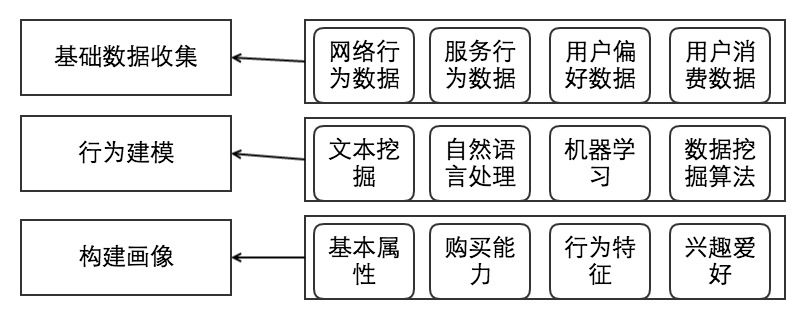
\includegraphics[scale=0.45]{figures/userprofile_process}}
	      \figcaption{用户画像的构建周期示意图}
	      \label{pic:userprofile_process}
	    \end{figure}
	    \begin{enumerate}[(1)]
	    \item 数据收集

	    数据收集大致分为四类:1、网络行为数据包括页面浏览量、活跃人数、访问时长、浏览注册转化率、注册活跃转换率等。服务内行为数据:点击浏览路径、网页停留时长、滑屏次数、滑屏频率、滑屏时长。用户内容偏好数据:点击、浏览、收藏内容、评价、评分、评论内容、社交内容、品牌偏好等。用户交易数据(交易类服务):购买率、折扣率、导流率、流失率等。收集到的数据没必要是百分之百的准确,大体差不多即可。应用中,具体就是在数据清洗阶段过滤一部分不靠谱的异常值,验证、更新数据这块需要在后面的阶段再做判断,比如某用户在性别一栏填的女,但其语言数据显示其为男的概率更大,根据业务再选择丢弃数据还是更新数据。
	    
	    \item 行为建模

	    该阶段是对收集到数据进行建模,目标是抽象出用户的文本标签,这个阶段不应该再纠结数据的正确性,而是应该注重大概率事件,通过统计学假设检验尽可能地排除用户的偶然行为。这时也要用到数据挖掘算法模型,对用户的行为进行回归预测,比如已有一个线性回归函数:y=kx+b,X 代表用户行为,y是函数拟合的用户喜好度,y'是用户真实偏好,我们通过不断的训练数据,利用参数k和参数b来得出最新损失函数下的值,用以精确模拟y'。

	    \item 用户画像基本成型

	    该阶段是行为建模的深化,需要利用用户的基本属性,如性别、地域、年龄,得出用户更高层的抽象概念:消费能力、忠诚度、活跃度、社交爱好等。因为用户画像永远也无法百分百地拟合现实中的一个人,只能做的就是不断地去减小拟合的损失函数,因此,用户画像需要根据变化的基础数据不断修正已有的更高层的抽象概念,尽可能模拟用户的变化趋势。

	    \item 数据可视化

	    最后是数据可视化分析,这部分是最能体现推荐系统的产出,因为人类对数据不如对图画来的敏感,在此步骤中一般是针对群体做进一步的抽象,按照消费习惯、消费能力、消费偏好把用户归类为一类人,比如可以根据用户对价格的敏感度细分出高价值用户、核心用户、高忠诚用户。而决策层所做出的评估也应该是基于某一群体的分布规律。典型的用户画像如\autoref{pic:user_profile}。
	    \end{enumerate}
		\begin{figure}
	    \centering
	      \framebox{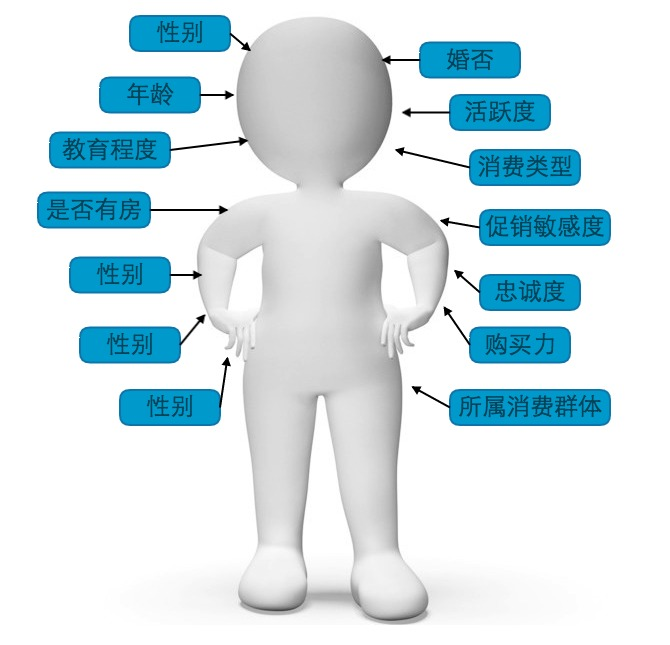
\includegraphics[scale=0.4]{figures/user_profile}}
	      \figcaption{用户画像示意图}
	      \label{pic:user_profile}
	    \end{figure}

		\subsection{用户画像的建模}
		用户画像的建模包括内容标签化和标签权重量化。建模过程:1、内容分析,从原先的物品描述信息中提取有用的信息用一种规范化的标签表示,有时候这种信息源自于作者提供的描述,有时候源自于用户的评价,不管如何,都需要人工做进一步的审核;2、上传、记录用户注册信息,生成用户基本信息,这些信息基本是不会变化的;上传、记录用户行为数据,这些数据是不断变化着的,通常是采用数据挖掘算法从潜在物品集合中取出若干个结果表示用户喜好的模型。例如,一个网页推荐系统,可以通过分析用户过往浏览过的文章,得出用户喜欢浏览类似于范冰冰的花边新闻,如果用户点击了所推荐的文章,则说明分析正确,否则需要根据反馈重新训练模型,从而实现一个反馈-推荐-反馈的闭环;3、推荐系统得出推荐集合后往往需要取topN,因为推荐系统的本质在精不在多。通过定义一个距离算法,匹配用户标签和商品标签的相关度,相关度一般正则为0-1之间,结果是一个二元的离散量:(pid, score)。根据相关度将生成一个用户潜在感兴趣的物品评分列表,然后去掉用户之前看过的商品,取topN即可。例如在电影用户画像的建模中,首先分析用户打分比较高的电影的共同特性,包括导演、演员、风格等,这些电影的标签就会成为此用户画像的一部分,根据打分的多少,给定一个合适的权重值。用户-标签用矩阵A表示,电影-标签用矩阵B表示,A乘B得出矩阵C,C代表了用户与电影之间的相关度,固定一个用户,对所有相关度不为零的电影做排序,取topN即是推荐结果。用户画像建模的根本在于用户标签的获取和权重的定量分析。

		对于商品描述,也可以做进一步的处理,丰富商品的标签集合。其实和文本处理类似,笔者选择使用目前应用最广泛的方法:TF-IDF方法。设有N个文本文件,关键词$k_{i}$在$n_{i}$个文件中出现,设$f_{ij}$为关键词$k_i$在文件$d_j$中出现的次数,那么$k_i$在$d_j$中的词频TF$_{ij}$定义为:TF$_{ij}$=$f_{ij}$/max$_zf_{zj}$,其中分母中的最大值是通过计算这个文本j中所有关键词出现的频率得出。附图给出了3个短文和5个关键词,以关键词人为例,该关键词在文本1中出现了1次,而文本1中出现次数最多的关键词是事,一共出现了2次,因此TF$_{11}$=0.5。一个关键词经常在许多文件中出现,则该关键词能表示文件的特性的意义就会较小,试想我们考察关键词i出现次数的逆,也就是$IDF_{i}$=log(N/$n_{i}$),这个想法和Adamic-Adar指数思路基本相似,关键词i在文本文件j中的权重于是可以表示为$w_{ij}$=$TF_{ij}$*$IDF_{i}$,而文件j可以用一个向量$d_{j}$=($w1_{j}$,$w2_{j}$,…,$wk_{j}$),其中k是整个文本库中关键词的个数。一般而言,向量应该是一个稀疏向量,即其中很多元素都为0。如果把用户今日点击、浏览、购买的商品抽象成一个标签向量,则可以通过用户标签向量-商品标签向量的点乘得出一个数值,从所有数值中把相似性最大的那个产品的标签更新给该用户画像,第二大相似性的产品标签权重减半更新给该用户画像,以此类推,完成用户画像的建模过程。
		\begin{lstlisting}
		文本1:不做软事,不说硬话,对事不对人。
		文本2:多少事,从来急;天地转,光阴迫。一万年太久,只争朝夕。
		文本3:青春之所以幸福,就因为它有前途。

		关键字包括人、事、硬话、一万年、朝夕、青春、幸福、前途
		\end{lstlisting}

		\subsection{用户画像和推荐系统的评测}
		首先,用户画像作为一个工具,只用在运用到某一场景才有意义,并能评估出其产出,因此本节主要介绍推荐系统的评测,根据推荐系统的表现好坏才能评估出用户画像的推荐质量。实际工程中,笔者利用A/B实验对若干组模型进行定量对比。标准的A/B实验是指通过一定的规则把类似的用户群随机分成俩组,采用旧模型的分组叫对照组,采用新模型的分组叫实验组\citep{ab-test}。通过对用户展示不同的模型,得出用户的使用指标,关键是各种转化率,这样仅仅通过对比倆者的转化率即可得出各个模型的优劣。策略实验的难点在于如何找到合适的实验设计方案。通过时间交错能够在一定程度上减少由时间片带来的误差,这样就有一个难题:  如何选择合适长度的时间片。策略实验往往伴随着携带效应(carry-over effects),也就是上一个时间片的策略会对下一个时间片带来影响。笔者和同事们提出一个方案,当选择适当大的时间片的时候,通过A/A实验的数据调整A/B实验的结果,具体来说,如果A/A实验的结果是 0.4\%, A/B实验的结果是 1.2\%。那么我们认为A/A实验是真实的时间片之间的差异, 我们需要用倆者之差的绝对值去调整时间片带来的影响,

	\section{用户画像在推荐系统的应用现状}
	Amazon的仓库里堆着数百万图书,Netflix的服务器中存储有数万部电影,淘宝平台上的小卖家总共拥有8亿件物品,除此之外,这三家公司都保留有数以亿计的用户行为数据。互联网电子商务开始积累了海量的用户数据,然后因为数据量过于庞大,有用信息如金矿中的金子一样很难挖掘利用,与此同时,用户发现常常需要面对过多的选择。心理学研究证实过多的选择会使人犹豫不决,导致消极等待,最终可能放弃消费的决定,这个问题严峻到可以造成肉眼可见的用户流失。近代统计学理论的发展加上最近几年的数据科学和数据挖掘工程的进步,为电子商务平台提供更有效的应对方案:推荐算法。推荐系统在帮助用户解决信息过载问题的同时,提升了企业价值。如今的企业不再局限于传统的推荐功能,通过建立完备的用户画像,推荐系统可以帮助企业更了解用户,在推广、反作弊、精细化运营等领域中发挥重要的作用。
		\subsection{基于用户画像的推荐系统的商业应用}
		\begin{figure}
	    \centering
	      \framebox{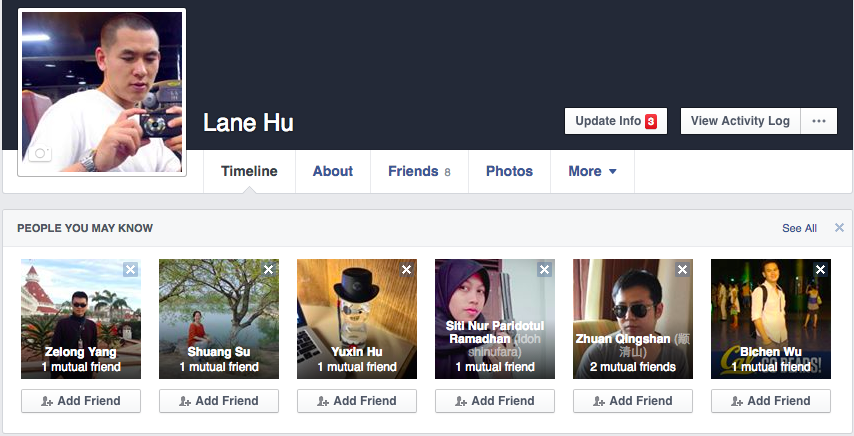
\includegraphics[scale=0.45]{figures/recmd_facebook}}
	      \figcaption{Facebook个性化推荐用户界面}
	      \label{pic:recmd_facebook}
	    \end{figure}
		作为全球社交网站中的翘楚,Facebook在很早的时候就预言到了大数据+推荐系统+用户画像的无限前景。Facebook自己的推荐系统就是需要利用分布式计算框架快速的帮助用户找到他们可能感兴趣的人、文章、分析、用户组等。Facebook是个伟大的公司,一直为开源软件贡献着一份力量,最近在其官网就公布了Facebook自己的推荐系统原理、性能及使用情况\citep{recmd-facebook}。Facebook的推荐系统需要面对的数据量应该是所有互联网公司中的数一数二,约包含了1000亿级别的评分数、10亿级别的用户数以及百万级别的虚拟商品,如何在如此庞大的数据规模下,仍然保持良好性能已经成为世界级的难题,而Facebook解决了,通过分析Facebook给出了一些实验的结果,表明,Facebook的系统比传统系统要快10倍左右。目前,该方法已经用到Facebook的多个app应用中,包括用户、用户组的推荐。Facebook推荐主页如\autoref{pic:recmd_facebook}。
		
		Facebook的用户画像进展也十分可观,几乎是与推荐系统同步发展。2011年12月,Facebook发布了里程碑式的大数据产品——Timeline,通过开发API接口,允许用户自行编辑个人的时间轴:在什么时间、什么地点做了什么,遇到了谁,可以说在这条时间线记录这个人的全部生活故事。Timeline通过帮用户回忆自己的点点滴滴的同时,完成了用户数据捕获、存储,而一旦拥有了这些历史数据,Facebook就可以做进一步的数据分析、挖掘,这时的Facebook就如同和你从小长大的小伙伴,一个懂你的陌生人。可以说用户留下的数据越多,Facebook就越了解这个人,投放的广告就会更加精准,最终Facebook利用庞大的用户数据生态赚足了钱。

		\subsection{推荐系统的主要方法}
		推荐系统主要有俩种思路:评分预测和Top-N预测,核心的目标都是找到最适合用户的候选集合s,从候选集合里挑选目标集合是一个非常复杂的非线性优化问题,通常采用的方案是用局部最优近似非线性最优,通过定义一个的损失函数,选取Top-N	\citep{recmd-Next}。

		推荐系统的算法基于统计学、概率论、线性代数、微积分技术,找出用户最有可能喜欢的商品,应该是现代互联网电商的明星应用。目前用的比较广泛的推荐算法还属协同过滤推荐算法,其基本思想是根据与他兴趣相近的用户的选择,得出推荐商品候选集,取topN推荐给目标用户,用维度为m×n的矩阵表示所有用户对所有物品的兴趣值,这个值应该是根据用户历史行为数据得出,值越高表示这个用户越喜欢,利用特殊值0表示没有接触过。图中行向量表示某个用户对所有商品的喜爱程度,列向量表示某个商品对所有用户的吸引程度,因此单个元素$U_{ij}$表示用户i对物品j的喜欢程度。协同过滤分为两个阶段:预测阶段和推荐阶段。预测阶段是基于所有原始集商品,预测这个用户有没有可能对其感兴趣,量化为一个数值,只要值不为零即可归为候选集中;推荐是根据预测结果,先去重后去除消费过的商品,然后取去TopN推荐给用户。

		尽管有这么多的优点,协同过滤算法也存在两大问题:1、数据稀疏性。一个大型的电子商务平台一般有百万级别的物品,用户可能接触到的商品占所有商品的百分之一不到,因此用户之间购买过的物品重叠性非常小,以至于没办法做推荐,一个办法是利用算法添补部分值\citep{recmd-slopone}。2、扩展性较差,因为一般来讲,电子商务平台中的商品变动很小,用户流入流出、日益增加、变动很大,基于用户的协同过滤算法需要不停的跟新迭代保证跟上用户变动的步伐。遇到这种情况,可以考虑基于商品的协同过滤算法,其基本思想类似于基于用户的协同过滤算法,只是相似性计算对象是商品,而商品一般变动很小可以忽略不计。如果我们知道物品a和b相似,而一般喜欢a的用户也喜欢b,如果用户A喜欢a,那么我们有很大把握得知A也应该喜欢b,推荐了准没错。而物品之间的相似性比较固定,因此可以一次性计算出物品的相似度,将结果存储到Redis中,推荐时查询Redis即可。

	\section{本章小结}
	本章简单概述了用户画像的研究现状,讨论了相关的建模过程,并从商业应用和学术研究两个角度介绍了推荐系统研究的现状,最后提到推荐系统的主要任务和面临的问题。
  %
\chapter{手机主题推荐系统整体设计与实现}
    \section{引言}
    小米主题应用拥有成千上万款主题包,而一个用户整个活跃周期只能接触不到十分之一的主题,所以我们现在面临的一个问题是,如何帮助用户发现新的主题,这些主题同时满足俩个条件:1、不能和用户之前看过的、购买过的主题包重复。2、不能和用户之看买过的、购买过的主题不相关,而这也是我们开发的手机主题推荐系统所要达到的目标之一。除此之外,手机主题推荐系统要达到的目标之二是帮助第三方设计师推广其作品。手机主题应用本身既不生产主题包,也不消费主题包,存在的价值就在于提供一个平台,能让用户、设计师和广告商从中受益。每个设计师都希望更多的用户体验、使用他们的主题。得益于个性化推荐系统的投入使用,我们现在可以把更多的主题包直接推送给那些潜在消费者面前。

    本章节主要介绍如何介绍手机主题推荐系统的完整架构。手机主题推荐由推荐模块、用户画像模型、用户兴趣探索模块组成。推荐过程流程为:首先,推荐系统把用户画像模型中兴趣需求信息和推荐主题模型中的特征信息匹配,然后使用排序算法进行计算筛选找到用户可能感兴趣的推荐主题,最后推荐给用户。
    \section{手机主题推荐系统设计}
    
    \begin{figure}
      \centering
        \framebox{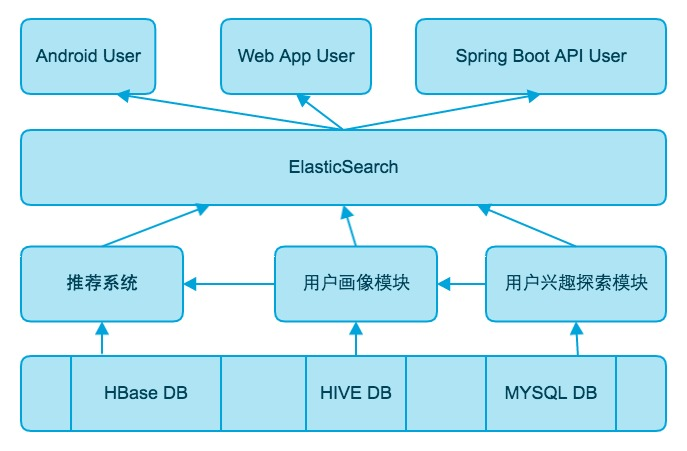
\includegraphics[scale=0.6]{figures/construct}}
        \figcaption{推荐系统引擎框架总览图}
        \label{pic:construct}
    \end{figure}

    推荐系统框架如\autoref{pic:construct}。最顶层显示的是推荐系统对外服务的客户端。由于不同展位的输入输出参数差异较大,因此这一层没有做过多的抽象,每个展位有自己特定的接口Json定义,接口层通过调用ElasticSearch搜索服务引擎实现秒级别的用户推荐结果列表。推荐系统利用离线方式更新ElasticSearch搜索服务器数据。用户画像模块除了作为推荐系统的输入数据外,也可以直接作为ElasticSearch的输入。用户兴趣探索模块定期扫描活跃用户和上架主题包,通过分析用户行为日志更新用户画像。从接口层接受到的每次响应请求会被记录成用户行为数据,包括请求的一些必要的上下文信息以及用户及主题包的特征信息。借助HBase、Hive、Mysql等数据平台对原始日志进行处理,从而得到需要的各种数据及模型:包括用户的画像信息,用户之间的相似度,商品之间的相似度。在推荐系统的候选集生成这一块,重度使用了item-based协同过滤算法,协同过滤算法需要在用户行为较丰富的情况下才能奏效。而对于那些行为稀少的用户和新用户,需要根据平台的特点进行做好冷启动策略。
    对于Spring Boot API User输入、输出数据格式分别如\autoref{code:api_input}和\autoref{code:api_output}所示。\\\\
    \begin{lstlisting}[language=json,firstnumber=1,label={code:api_input}]
      {
        "user_id":"123",
        "dims":{"type":"normal", "free_or_charge":"mixed"},
        "white_list":{"id":1141},
        "max_number":"8",
        "start_date":"2016-07-01,
        "end_date":"2016-08-01
      }
    \end{lstlisting}

    \begin{lstlisting}[language=json,firstnumber=1,label={code:api_output}]
    {
      "code":0,
      "message":"successfully",
      "data":{
        "total":111,
        "themes":[{
          "id":1141,
          "subscribe":1,
          "business":null,
          "keytype":"market:orderid",
          "tag":null,
          "name":"lovely baby",
          "displayName":"小可爱",
          "description":"家庭,儿童欢乐多",
          "author":"摆渡车1024",
          "sigModel":2,
          "type":2,
          "dependency":null,
          "createTime":1462447261000,
          "dims":null}
        ]}
    }
    \end{lstlisting}

    \subsection{数据采集和日志格式化}
    我们的数据采集来源包括有移动端埋点和用户请求。目前常见的前端埋点技术有三类:代码触发埋点、可视化触发埋点和延迟埋点,根据手机主题商店的业务特点和用户规模,我们选用可视化触发埋点,当用户在UI上点击了某个可埋点的控件时,会自动触发回调函数调用接口发送相应事件的log信息,可视化触发埋点不同于代码触发埋点,其理念是把核心代码和配置、资源分开,在APP启动的时候通过网络更新配置和资源即可,不必每一个埋点都需要写代码,埋点产生的数据量很少,且只针对特定人群,所以用来做A/B测试的数据源。用户请求每一次行为都会被上传、存储到服务器。获取数据后根据数据来源和存储方式,将日志格式化为:public日志、nginx日志、binlog日志和passport日志,public日志存放手机端用户请求log,nginx日志存放Web端用户请求,binlog日志是将Mysql内容同步到NoSQL DB的数据,passport日志存储用户验证信息等数据。

    \subsection{用户画像的收集}
    当上述日志格式化生成,通过每日定时任务扫描passport日志就可以获取新注册用户并为其在ElasticSearch创建一个topic,同时利用移动端埋点功能获取到用户手机IMEI号、经纬度等基本信息,利用用户注册手机号或者邮箱账号获取用户的通信录和好友信息,借助好友信息完善此用户的用户画像,除此之外有时可以借助第三方接口获取用户的基本信息。用户画像的构建相对来说比较简单,只涉及到标签产出,没有权重量化。

    \subsection{商品标签的构建}
    小米手机主题应用商店里的主题包大多数是由第三方设计师创建、当设计师上传成品到官方产品库时会被要求填写作品标签,官方审核员也会更改、删除、添加一些标签,作品上架后用户在浏览、购买时产生的评论文本也会生成一些标签,商品标签的构建也只涉及到标签生成,没有产生权重。

    \subsection{候选集的生成}
    通过用户与商品的交互行为矩阵,我们最终得到了带有标签权重的候选集,具体算法是利用Item-based协同过滤算法生成候选集,定义N$_u$表示用户u之前喜欢的主题集合,则用户u对主题i的偏好度根据\autoref{ItemCF}可计算得到。
    \begin{equation}
    p(u,i)=\sum \limits _{j\in N(u)}^{} r(u,j)s(i,j)
    \label{ItemCF}
    \end{equation}

    其中,r$_{u,j}$表示用户u对主题j的偏好度,s$_{i,j}$表示主题i和主题j之间的相似度。Item-based协同过滤算法定义俩个主题之间的相似度由集中在这个俩个主题的用户行为数据计算得出。N$_{i}$为看过主题i的用户集合,N$_{j}$为为看过主题j的用户集合,因此,主题i和主题j的相似度计算公式为\autoref{Item-item-similar}
    \begin{equation}
    s(i,j)=\frac{\left | N(i)\cap N(j) \right |}{\sqrt{\left | N(i) \parallel N(j) \right |}}
    \label{Item-item-similar}
    \end{equation}

    根据\autoref{Item-item-similar}可知,如果有很多用户同时看了主题i和主题j,那么主题i和主题j之间的相似度就会很高,不幸的是,这也会导致所有热门主题之间的相似度都很高,导致推荐结果包含热门主题包过多。我们的解决思路是对热门主题包降权,同时控制热门主题所占比例。

    \subsection{排序}
    排序主要是对候选集的生成的标签权重做排序,但会加入一些倾斜因子,如用户活跃度、主题包的热度、经纬度等因子,最终根据标签权重+倾斜因子的排序得到推荐结果。

  \section{用户画像与用户兴趣探索}
  众所周知用户的需求是动态变化着的,不管是随着季节周期性变动,还是随着年龄发生非逆转变化,都意味着一些标签需要删除掉,一些标签需要加进来。用户画像的数据来源包括:原始的用户行为数据和用户兴趣探索模块,前者只是更新那些显而易见的标签,而后者负责在海量数据中挖掘出那些稍纵即逝的用户行为并准确分析用户的意图,由此可见用户兴趣探索对活跃用户效果相对较好,并且针对小众主题包进行挖掘的效果很棒,可以明显提升推荐结果的多样性。除此之外,我们利用基于时间窗口的遗忘机制解决了将新发现的用户兴趣和原有兴趣合并为用户的新兴趣的问题,时间窗口机制与自然遗忘规律相似,排前面的标签时效性最好,排后面的标签时效性差,将会被优先淘汰。通过设置时间窗口的大小、时间窗口的滑动速率,可以间接控制新、旧兴趣的比例。

  \section{用户画像与推荐系统}
  一个好的推荐系统要给用户提供个性化的、高效的、动态准确的推荐,那么推荐系统应能够获取反映用户多方面的、动态变化的兴趣偏好,推荐系统有必要为用户建立一个用户兴趣探索模型,该模型能获取、表示、存储和修改用户兴趣偏好,能进行推理,对用户进行分类和识别,帮助系统更好地理解用户特征和类别,这就是我们要引进用户画像的根本原因。用户画像模块和兴趣探索模块的关系如\autoref{pic:hl_iterate}所示。
  \begin{figure}
    \centering
      \framebox{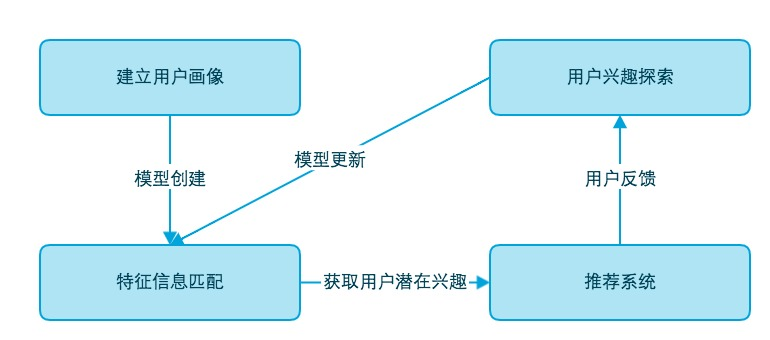
\includegraphics[scale=0.4]{figures/hl_iterate}}
      \figcaption{用户画像数据流图}
      \label{pic:hl_iterate}
  \end{figure}

  一个好的用户画像需要有一个完整的标签体系,包括标签的数量、质量和粒度。其中标签的数量直接影响推荐系统的结果完整度,标签的质量直接影响推荐系统的精度,而标签的粒度会影响推荐系统的用户满意度。完善的标签体系更像一个金字塔,一级是最基本的概念标签,如动漫、运动等,数量被控制在几十个左右,二级标签是上层标签的扩展,如美少女动漫、搞笑动漫、篮球运动、足球运动,三级标签就是指具体化了的标签,如街头篮球、NBA篮球、CBA篮球等。对于活跃度高的用户标签倾向于下沉,推荐结果数据多、精度高,活跃度低的用户反之。对于一个新创建的用户画像,刚开始只包含最基本的用户人口信息,随着用户行为数据的累积会逐渐丰富起来。

  \section{本章小结}
  本章首先介绍了整个推荐系统结构,然后介绍了数据集的生成、格式,以及基于数据集的用户画像建模和商品标签建模,最后介绍了用户画像和用户兴趣探索,用户画像和推荐系统中的交互关系。
   
\chapter{用户画像模块}
\section{引言}
\label{chap:example}
Alan Cooper最早提出了用户画像的概念:Personas are a concrete representation of target users。Persona 是真实用户的虚拟代表,是建立在一系列真实数据之上的目标用户画像。通过用户历史行为去了解用户,根据他们的目标、行为和观点的差异,将他们区分为不同的类型,然后每种类型中抽取出典型特征,赋予名字、照片、一些人口统计学要素、兴趣标签等描述,就形成了一个人物原型,\autoref{pic:hl_userProfile}所示为一个典型的用户画像,标签面积越大代表其权重越高。

刻画每个用户,是任何一家社交类型的服务都需要面对的问题,不同的公司针对各自业务会有不同的需求,构建用户画像的动机和目标也会存在一定差异。从手机主题应用的业务特点来讲,构建用户画像的目的包括:

\begin{figure}
\centering
  \framebox{\includegraphics[scale=0.35]{figures/hl_userProfile}}
  \figcaption{用户画像标签示例图}
  \label{pic:hl_userProfile}
\end{figure}

\begin{itemize}
\item 完善及扩充用户信息:用户画像的首要动机就是了解用户,这样才能够提供更优质的服务。但是在实际中用户的信息提供得不尽完整,如对于没有填写性别信息的用户,用户画像通过分析用户语音数据识别其性别,尽可能多的为推荐系统提供正确的基础特征。
\item 打造健康的主题设计生态圈:在掌握用户信息的基础上,平台就可以对自身的状况进行分析,从相对宏观的基础上把握主题市场的生态环境,挖掘设计作品的最大价值,帮助设计师提高收入。例如通过对用户信息的聚类,能够对用户进行人群的划分,掌握不同人群的活跃程度、行为及兴趣偏好,热门主题的传播方式和流行引爆点等。
\item 支撑主题推荐系统的精准推荐:精准推荐的前提是对用户的清晰认知。以简单代金券发放为例,手机主题应用市场的历史数据呈现出两大类四种不同的消费习惯。代金券敏感型:发代金券才用、发代金券用的更多;代金券不敏感型:发不发都用,发代金券也不用。在推荐系统的用户画像系统中,上述四种群体会被分别冠以屌丝、普通、中产、土豪的标签。针对四类用户的运营策略也会全然不同,最直接的就是代金券的刺激频率以及刺激金额,而对“代金券”免疫的土豪群体,则更多地需要在优化服务上做文章。在实际场景中,影响用户对手机主题包的使用黏度的因素要远比代金券复杂得多,在这种情况下,利用用户画像可以对用户的“贴身跟踪”就能及时发现薄弱环节,因此从用户打开应用商店到退出使用,其间的每一步情况都被快的记录在案:哪一天退出的,哪一步退出的,退出之后“跳转”到什么软件等等。据此,用户画像也实现了用户另外一个纬度的归类,分清哪部分是忠实用户,哪部分可能是潜在的忠实用户,哪些则是已经流失的;更进一步来看流失的原因:因为代金券没有了流失?主题包质量不好流失?这些都是下一步精准推荐的依据,无论是基于兴趣的推荐提升用户价值,精准的广告投放提升商业价值,还是针对特定用户群体的内容运营,用户画像都是其必不可少的基础支撑。直接地,用户画像可以用于兴趣匹配、关系匹配的推荐和投放;间接地,可以基于用户画像中相似的兴趣、关系及行为模式去推动用户兴趣和设计师的无缝对接。
\item 主题市场安全领域的应用:随着手机主题市场的发展,商家会通过各种活动形式的补贴来获取用户、培养用户的消费习惯,但同时也催生一些通过刷排行榜、刷红包的用户,这些行为距离欺诈只有一步之遥,但他们的存在严重破环了市场的稳定,侵占了活动的资源。其中一个有效的解决方案就是利用用户画像沉淀方法设置促销活动门槛,即通过记录用户的注册时间、历史登陆次数、常用IP地址等,最大程度上隔离掉僵尸账号,保证市场的稳定发展。
\end{itemize}

    \section{用户画像数据类型}
    在个性化服务的用户画像建模中,一个完整、成熟的用户画像应该包含基础静态数据类型、基础行为数据类型和高维数据类型。
    \subsection{基础静态数据类型}
    当一个新用户注册时会填写人口基本信息,通过json格式从客户端传回服务器,格式如
    \begin{lstlisting}[language=json,firstnumber=1]
        {"registerLog": {
          "userId": "001",
          "gender": "male",
          "profession": "student",
          "phone": "null",
          "borthday": "19860820",
          "isWeiboUser": "no",
          "isWeixinUser": "yes",
          "city": "北京市",
          "timestamp": "1453700393",
          "...": "..."
        }}
    \end{lstlisting}
    有的用户会利用微信、微博提供的第三方免登陆API,第三方数据可以用来交叉验证用户填写的基础信息数据。用户每次登陆时应用程序还会获得其手机品牌、操作系统等信息。因此,通过解析server log得到基础静态数据形式:
      \begin{table}[htp]
      \centering
      \tabcaption{用户-基础静态数据矩阵表}
      \label{tab:tagweight}
      \begin{tabular}{|c|c|c|c|c|c|c|c|} \hline
       用户id & 性别 & 年龄 & 职业 & 电话号码 & 手机运营商 & 是否为微博用户 & ... \\ \hline
       001 & 女 & 23 & 学生 & 13948572214 & 移动 & 是 & ... \\ \hline
       002 & 男 & 30 & 学生 & 15811036703 & 移动 & 是 & ... \\ \hline
       ... & ... & ... & ... & ... & ... & ... & ... \\ \hline
      \end{tabular}
      \end{table}

    \subsection{基础行为数据类型}
    基础行为数据是指用户的一些行为,包括购买,试用,浏览,评价等的统计量,用户行为数据格式如
      \begin{lstlisting}[language=json,firstnumber=1]
        {"actionLog": {
          "userId": "001"
          "actions": [{
              {"itermId": "0822"},
              {"actionType": "jumpIn"},
              {"stayTime": "32000"},
              {"clickNum": "2"},
              {"scrollNum": "5"},
              {"timestamp": "1453701393"},
              {"...": "..."}
          }]
        }}
      \end{lstlisting}
    基础行为数据作为用户行为统计量可以反映用户的活跃度、消费能力和用户类型。基础行为数据形式如:
      \begin{table}[htp]
      \centering
      \tabcaption{用户-基础行为数据表}
      \label{tab:tagweight}
      \begin{tabular}{|c|c|c|c|c|c|c|c|} \hline
       用户id & 购买 & 试用数 & 浏览 & 未支付订单数 & 活跃时间段 & 日浏览时长 & ... \\ \hline
       001 & 2 & 7 & 118 & 0 & 20:00-22:00 & 120 & ... \\ \hline
       002 & 0 & 3 & 7 & 1 & 13:00-14:00 & 60 & ... \\ \hline
       ... & ... & ... & ... & ... & ... & ... & ... \\ \hline
      \end{tabular}
      \end{table}

    \subsection{高维数据类型}
    高维数据是用户画像模型从基础静态数据和基础行为数据统计、分析、抽象出来,用来衡量用户某一方面的价值,如用户信用是指是否有过作弊行为、退款次数过多等综合评估,用户价值是指购买次数、单笔消费额、消费频率的综合评估。高维数据可以用矩阵来表示:
      \begin{table}[htp]
      \centering
      \tabcaption{用户-高维数据表}
      \label{tab:tagweight}
      \begin{tabular}{|c|c|c|c|c|c|c|c|} \hline
       用户id & 信用 & 价值 & 忠诚度 & 活跃度 & 价格敏感度 & 奖励敏感度 & ... \\ \hline
       001 & 高 & 高 & 高 & 高 & 低 & 低 & ... \\ \hline
       002 & 中 & 中 & 高 & 高 & 高 & 高 & ... \\ \hline
       ... & ... & ... & ... & ... & ... & ... & ... \\ \hline
      \end{tabular}
      \end{table}

    \section{用户画像建模}
    用户画像建模的过程就是原始数据进过处理、分析得到可信度高的用户标签信息的过程,对于不同类型的用户数据其建模的侧重功能点也有所区别。
    \subsection{基础静态数据建模}
    用户基础静态数据的特点是数量不多,但在推荐系统中所占的权重较大,因此对其可信度要求较高,在对基础静态数据建模的时候主要实现俩个功能:根据上下文信息补全为为空的标签和根据上下文信息校验已有的标签。

    标签补全以用户性别标签为例,新用户注册时如未填写性别信息其值会默认设为Null,方便用户画像建模时判断。主要思路是通过分析用户上下文信息,包括第三方登入数据、用户语音和头像获得用户真实的性别,如以上方法都未成功获取用户性别,程序会利用线性回归算法挖掘出一个最有可能的性别标签值,代码:
    \begin{lstlisting}
      public String getUserGender(String log) {
          Gson gson = new Gson();
          UserProfile userProfile = gson.fromJson(log, UserProfile.class);

          if (userProfile.gender != null) {
              return userProfile.gender;
          }

          String useId = userProfile.useId;
          //通过第三方应用登陆数据得到用户信息
          UserProfile thirdPartUP = gson.fromJson(getThirdPartUserInfo(useId), UserProfile.class);
          if (thirdPartUP.gender != null) {
              return thirdPartUP.gender;
          }

          //通过分析用户语音数据得到用户信息
          UserProfile voiceUP = gson.fromJson(getUserVoiceUserInfo(useId), UserProfile.class);
          if (voiceUP.gender != null) {
              return voiceUP.gender;
          }

          //通过线性回归算法挖掘出用户信息
          UserProfile lrUP = gson.fromJson(getLinearRegressionUserInfo(useId), UserProfile.class);
          return lrUP.gender;

      }
    \end{lstlisting}

    标签校验是指虽然相关信息已经被填写,但程序认为其值具有随意性,需要根据上下文信息加以确认并校验,标签校验由于考虑的因素较多导致计算量大,使得其应用场景较少,还是以用户性别标签为例,代码:
    \begin{lstlisting}
        public String getRightUserGender(String log) {
        int[] count = {0, 0};
        Gson gson = new Gson();
        UserProfile userProfile = gson.fromJson(log, UserProfile.class);

        if (userProfile.gender != null) {
            if (userProfile.gender.equals("male")) {
                count[0]++;
            } else {
                count[1]++;
            }
        }

        String useId = userProfile.useId;
        UserProfile thirdPartUP = gson.fromJson(getThirdPartUserInfo(useId), UserProfile.class);
        if (thirdPartUP.gender != null) {
            if (thirdPartUP.gender.equals("male")) {
                count[0]++;
            } else {
                count[1]++;
            }
        }

        UserProfile voiceUP = gson.fromJson(getUserVoiceUserInfo(useId), UserProfile.class);
        if (voiceUP.gender != null) {
            if (voiceUP.gender.equals("male")) {
                count[0]++;
            } else {
                count[1]++;
            }
        }

        UserProfile lrUP = gson.fromJson(getLinearRegressionUserInfo(useId), UserProfile.class);
        if (lrUP.gender.equals("male")) {
            count[0]++;
        } else {
            count[1]++;
        }
        if (count[0] >= count[1]) {
            return "male";
        } else {
            return "female";
        }
    }
    \end{lstlisting}

    \subsection{基础行为数据建模}
    基础行为数据建模跟新频率较快,计算量较大,因此采用离线方式利用sql语句从hive表中得出用户在一段时间区间内特定行为的统计数据。需要注意一些用户行为的延迟性,如购买行为,从下单到支付成功可能跨越若干天,因此约定订单量以支付时间为准,有时候遇到网络故障相同订单会被用户提交多次,需要利用distinct做去重操作。统计特定用户某段时间的订单量的sql语句:
    \begin{lstlisting}
      set hiveconf:ymdwithline=2016-04-06;
      set hiveconf:userId=525108009;

      select count(distinct a.order_id) score
      from theme_dw.dw_v_order_base
      where concat_ws('-',year,month,day) between date_sub('${hiveconf:ymdwithline}',5) and '${hiveconf:ymdwithline}'
      and userId='${hiveconf:userId}'
      and finish_time like '${hiveconf:ymdwithline}%'
    \end{lstlisting}

    \subsection{高维数据建模}
    高维数据建模的数据来源包括基础静态数据、基础行为数据,数据类型包括累计量和趋势量,累计量包括用户浏览总数、用户购买总数等,趋势量是指用户最近登录时间、最近购买时间等,利用数据挖掘分类算法得出一个训练模型,需要注意的是用户行为类型、发生时间、发生位置会影响模型的权重计算,即weight = (行为类型 + 时间上下文 + 空间上下文) × 时间衰减因子。其中,用户行为类型包括浏览、购买、搜索、评论、购买、点击赞、收藏等,我们定义购买权重计为5,而浏览仅仅为1。空间上下文是指用户跳转入口方式,我们定义搜索入口权重3,排行榜入口为2。时间上下文是指用户之前是否接触过此类标签,接触频率等。时间衰减因子根据半衰期公式得出,如所示\autoref{equ-half_life},其中T取值为1,t为行为发生时间距离当前时间的天数。
    \begin{equation}
      score=(\frac{1}{2})^{(t/T)}
      \label{equ-half_life}
    \end{equation}

    以用户活跃度为例,由于日活跃变动过大,月活跃过于滞后,因此按周统计,模型选择线性回归算法,模型输入为基础静态数据、基础行为数据,模型输出为一个int型整数,值为[1,2,3],分别对应不活跃、较活跃、活跃。代码:
    \begin{lstlisting}
      public int getActivityScore(String userId) throws Exception {
          String userBaseInfo = getUserBaseInfo(userId);
          String userActionLog = getUserActionLog(userId);
          Gson gson = new Gson();
          String score = getLinearRegressionActivityScore(gson.fromJson(userBaseInfo, UserProfile
                  .class), gson.fromJson(userActionLog, UserActions.class));
          double activityScore = Double.parseDouble(score);
          if (activityScore >= 66) {
              return 3;
          } else if (activityScore >= 33) {
              return 2;
          } else {
              return 1;
          }
      }
    \end{lstlisting}

    \section{实验与分析}
    本节的研究目标是如何利用用户画像给新注册用户做出准确的Top-N推荐并提升用户留存率。
      \subsection{数据集准备}
      手机主题应用月新注册用户超过20万个用户,大部分用户的第一个月的行为记录少于10个,我们从2015年9月1号到2015年9月7号这段时间,筛选出所有注册信息相对完整的用户数据作为实验数据集,create table 格式:
      \begin{lstlisting}[language=json,firstnumber=1]
        {
        //静态数据
        user_id                  int    comment '用户id',
        user_name                int    comment '用户name',
        user_age                 int    comment '用户age',
        create_time              string comment '账号创建时间',
        city_id                  int    comment '城市id',
        city_name                string comment '城市名',
        phone                    int     comment '手机号',
        os_version               stringt comment '操作系统及版本',
        phonetype_serial         string  comment '手机品牌及型号',
        education_level          string  comment '学历',
        school                   string  comment '学校',

        //行为数据
        click_num int comment '点击次数',
        last_click_time int comment '最近点击时间',
        buy_num int     comment '购买次数',
        last_buy_time int     comment '最近购买时间',
        try_use int     comment '试用次数',
        last_tryuse_time int     comment '最近试用时间',
        browse_num int     comment '浏览次数',
        last_browse_time int     comment '最近浏览时间',
        browse_total_time int     comment '浏览总时长',
        login_num int     comment '登陆总次数',
        login_total_time int     comment '登陆总时长',
        comment_num int     comment '评论总次数',

        //高维数据
        use_time                 int     comment '使用时间段',
        not_use_time             int     comment '沉默天数',
        friendship               list<bigint>  comment '好友关系',
        friend_group             list<bigint>  comment '好友圈',
        coupon_sensitivity_score decimal(20,4) comment '券敏感及阈值',
        purchase_will_score      decimal(20,4) comment '消费意愿',
        loyal_score              decimal(20,4) comment '忠诚度',
        credit_score             decimal(20,4) comment '活跃度'
        }
      \end{lstlisting}
      \subsection{评测指标}
      本节使用线上A/B测试方案\citep{ab-test},利用用户留存率来评测推荐系统应对冷启动问题的效果。用户留存数是指在某段时间开始使用App应用,经过一段单位时间后仍然继续使用该App应用的用户,用户留存率是指用户留存数占当时新增用户的比例,这里的单位时间取天,实验时间区间为2015年9月7号到2015年9月30号。用户留存率研究对象为新注册用户,反映了推荐系统的转换能力,即由初期的不稳定的用户转化为活跃、稳定、忠诚的用户。
      \subsection{对比模型}
      基准模型为融合了用户画像的推荐模型,对照模型为单纯的推荐模型和推荐热门商品的简单推荐模型。每个推荐模型分流10\%的用户流量,推荐算法使用了开源软件spark MLlib的LogisticRegressionWithLBFGS模块,前俩个模型的推荐候选集为全部主题,简单推荐模型的推荐候选集为top20\%热度的主题。我们对比了单纯的推荐模型、推荐热门商品的简单推荐模型和融合了用户画像的推荐模型在2015年9月新注册用户数据集上的用户留存率。\autoref{pic:hl_saveRatio}展示了不同模型的实验结果。图中,横坐标是时间变量,单位为天,纵坐标是用户留存率,每一条曲线代表了一个模型的用户留存率随时间变化的曲线。通过观察曲线可以发现用户留存率随时间流动呈指数分布,头三天就流失了约90\%的新用户,从第四天用户留存率开始停留在一个比较稳定的阈值,实验结果显示,融合了用户画像的推荐模型相对其他模型有更高的留存率。截止到2015年9月30号,融合了用户画像的推荐模型的留存率是10.3\%,比推荐热门商品的简单推荐模型的留存率8.19\%高了2.11个百分点,相对于单纯的推荐模型的留存率5.76\%高了4.54个百分点。由此可见用户画像能够很好的解决冷启动问题并得到较高的新注册用户留存率。
      \begin{figure}
      \centering
        \framebox{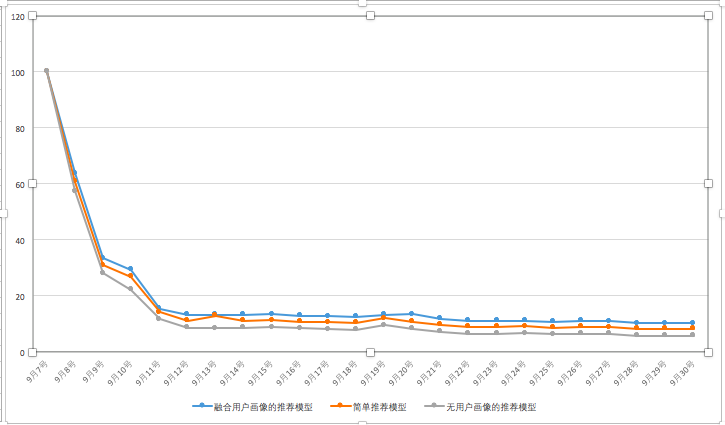
\includegraphics[scale=0.55]{figures/hl_saveRatio}}
        \figcaption{新用户留存率实验对比图}
        \label{pic:hl_saveRatio}
      \end{figure}

    \section{本章小结}
      用户画像对于推荐系统来讲,主要几个方面的提升:提升推荐系统的精度,用户画像将用户的长期偏好融入到了推荐内容中,维护了推荐系统一致性。abtest显示,融合了用户画像的推荐模型比单纯的推荐模型在点击转化率指标提高了约2.8\%,考虑到300万用户的基数,2.8\%的提升是一个很大的进步;用户画像还解决新用户的冷启动问题,对于一个新注册用户来讲,推荐系统可以利用用户画像的静态信息,然后结合商品信息进行推荐;提高推荐系统的时效性,对用户行为的离线预处理,可以节约推荐系统的大部分计算时间。但是用户画像只是反映了用户长期的兴趣,所以无法动态的反映用户短期兴趣,因此我们引入了用户兴趣探索模块,将在下一章节件详细介绍。

  %自行添加
  
\chapter{用户兴趣探索}
\section{引言}
\label{chap:interestExplore}
电子商务产品的设计往往是数据驱动的,即许多产品方面的决策都是把用户行为数据量化后得出的。但就小米主题市场而言,那些热门主题往往只代表了用户一小部分的个性化需求,只有通过对用户行为的充分分析,才能更好的挖掘出用户的兴趣,最终提升商品的销售量。现有的推荐算法注重用户或资源间的相似性的同时却忽略了用户兴趣的动态变化,从而导致系统在时间维度上有偏离用户需求的趋势。

探索用户兴趣的数据来源包括用户画像和商品特征表。用户画像包括用户基本信息和兴趣标签等,商品特征表包括分类、属性标签等,用户兴趣探索过程分为几个步骤:首先,利用用户历史行为(评论,停留时长,评分,点赞,购买等)量化用户满意度,然后利用用户兴趣特征向量与商品特征矩阵得出相关分数,如果商品与用户的相关分数很低,但有很高的用户满意度,说明是一次成功的用户兴趣探索,更新用户画像。如果是热门商品,大量的用户都会点击,但商品与用户不是很相关,则认为其探索效果是有限的,反之如果是小众商品,考虑到长尾效应,则可以认为其是更成功的兴趣探索。这里涉及到的概念包括用户满意度的量化、用户和商品的关联度、商品属性标签的长尾性。

\section{用户行为数据的存储和处理}
手机主题用户行为数据的特点包括:用户基数庞大。手机主题注册用户达千万级,活跃用户达百万级;用户规模增长快。月新注册用户达10万数量级。每个用户的行为数量较小。即使是活跃用户,每天最多也只产生上百条行为记录;用户行为的计算较为复杂。计算用户的两次登录间隔天数、反复购买的商品、累积在线时间,这些都是针对用户行为的计算,通常具有一定的复杂性;用户行为数据格式不规整,字段丢失率较高。根据用户行为数据的这些特点,我们采用基于HDFS分布式文件集群存储数据。

  \subsection{数据预处理}
  数据预处理是数据挖掘过程中一个重要步骤,主要工作包括字段去重、无效日志过滤、多表字段的连接等。如统计2015年09月06号userId为001的投诉数,数据预处理过程如\autoref{code:data-predoing}。
  \begin{lstlisting}[language=java,firstnumber=1,label={code:data-predoing}]
    set hiveconf:ymdwithline=2015-09-06;
    set hiveconf:metric=complaint_order_num;
    set hiveconf:user_id=001;

    select '${hiveconf:metric}' as metric, count(a.order_id) as score
    from (
        //去重
        select distinct order_id
        from theme.dw_v_order_base
        //以时间范围date_sub('${hiveconf:ymdwithline}',5) and '${hiveconf:ymdwithline}'为条件过滤掉不符合条件的订单
        where concat_ws('-',year,month,day) between date_sub('${hiveconf:ymdwithline}',5) and '${hiveconf:ymdwithline}'
        //无效订单过滤
        and order_id!=null
        //以用户id为条件过滤掉其他订单
        and user_id=${hiveconf:user_id}
    ) a
    inner join (
        //order_id 字段去重
        select distinct order_id
        from theme.g_comment_complaint
        //type = 3表示用户投诉
        where concat_ws('-',year,month,day) = '${hiveconf:ymdwithline}' and type = 3
        //多表字段的连接,如果有一个表有投诉记录,就算一次投诉。
        union
        select distinct order_id
        from theme.dwd_kefu_phone_complaint
        where concat_ws('-',year,month,day) = '${hiveconf:ymdwithline}'
    ) b
    on a.order_id = b.order_id
    inner join (
        select order_id
        from theme.pay_info
        where ymd = ${hiveconf:ymdwithline}
            //status=1代表当前订单状态为已支付
            and status=1
    ) d
    on a.order_id = d.order_id
    group by metric;
  \end{lstlisting}

\section{用户兴趣探索模型}
用户兴趣探索主要功能模块包括:1,兴趣标签探测,在分析用户行为数据时,如果某些主题标签是这个用户画像没有的,那么这些标签会作为标签探索候选集。2,长尾标签提取,遍历标签探索候选集,如果不属于小众标签集的标签将会被过滤掉。3,用户满意度量化,根据用户所有对某一个主题的行为数据得出这个用户对这个主题的满意度。4,标签权重的更新,不管是不是一次成功的兴趣标签探索,都要对用户画像标签的权重做更新,更新算法利用了线性衰减思想。本章首先介绍一些基本概念,包括长尾标签的定义、用户满意度的量化等。然后详细介绍用户兴趣探索功能模块的实现。
  \subsection{基本概念概述}
  实体域。如果一个模型是基于分析用户行为得出用户兴趣时,实体就是这个行为针对的对象。不同实体通过标签关联起来,对于手机主题应用市场来说,实体域还包括所有的背景图片,铃声,闹铃等。

  用户行为。包括浏览,点击,下载,试用,购买,评论。本文所指的用户行为都是指用户在某手机主题上的行为。
  
  用户兴趣。用户兴趣同样是限定在某实体域的兴趣,通常以标签+权重的形式来表示。比如,对于手机主题,用户兴趣向量可以是(动漫,0.6),(NBA,0.1),(性感,0.7)等分类标签。值得一提的是,用户兴趣只是从用户行为中抽象出来的兴趣维度,并无统一标准。而兴趣维度的粒度也不固定,如“体育”,“电影”等一级分类,而体育下有“篮球”,”足球“等二级分类,篮球下有”NBA“,”CBA“,”火箭队“等三级分类。

  兴趣空间。用户兴趣是在同一层次上兴趣维度的集合,比如手机主题中,可以用”热门“,”游戏“,”限时特价“,”科技“来构成一个程序员兴趣标签空间,也可以用”二次元“,”萝莉“,”魔幻“,”纯真“,”召唤兽“·····”法术“等构成一个动漫兴趣标签空间。

  小众标签集。小众标签集是指出现频率低的主题标签的集合,代码如\autoref{code:cold-tag}。
  \begin{lstlisting}[language=java,firstnumber=1,label={code:cold-tag}]
    public HashSet<String> getLongTailTags() throws Exception {
        Map<String, String> tagsCount = new TreeMap<>();

        //获取所有主题包
        Map<String, Object> allThemes = getAllThemes();
        for (Map.Entry<String, Object> theme : allThemes.entrySet()) {
            String themeName = theme.getKey();
            //获取当前主题的所有标签
            Object themeTags = ((Map<String, Object>) theme.getValue()).get("tags");
            for (String tag : (Set<String>) themeTags) {
                //出现一次,tag 对应的count加1
                tagsCount.put(tag, tagsCount.get(tag) + 1);
            }
        }

        //这里将map.entrySet()转换成list
        List<Map.Entry<String, String>> list = new ArrayList<Map.Entry<String, String>>(tagsCount
                .entrySet());
        //然后通过比较器来实现排序
        Collections.sort(list, new Comparator<Map.Entry<String, String>>() {
            //升序排序
            public int compare(Map.Entry<String, String> o1, Map.Entry<String, String> o2) {
                return o1.getValue().compareTo(o2.getValue());
            }
        });

        HashSet<String> out = new HashSet<>();
        //取频率最小的那80%标签作为小众标签
        double threshold = list.size() * 0.8;
        for (int i = 0; i <= threshold; i++) {
            out.add(list.get(i).getKey());
        }

        return out;
    }
  \end{lstlisting}

  用户满意度量化。用户满意度量化是指根据用户作用在主题上的不同行为动作及其参数值,参数值包括动作类型、次数和时长,得到一个衡量用户满意度的分数。

  标签集中度(tagFocus)。标签集中度是指如果某个标签在一类主题中出现的频率高,其他主题类型很少出现,则认为此兴趣标签具有很好的类别区分能力。这是因为包含兴趣标签t的主题越少,也就是n越小,则说明标签t具有很好的兴趣区分,则其探索权重越大。如果某一类主题包C中包含兴趣标签t的个数为tagInThemeNum,而其它类包含t的总数为tagInOtherNum,则所有包含t的主题数n=allThemeNum,当m大的时候,n也大,标签权重值会小,就说明该标签t类别区分能力不强。实际上,如果一个标签在一个类的主题中频繁出现,则说明该标签能够很好代表这类主题的特征,这样的标签应该给它们赋予较高的权重,并选来作为该类主题的特征向量以区别于其它类主题,标签集中度公式如\autoref{equ:focus},我们很容易发现,如果一个标签只出现若干主题包,我们通过它就容易定位搜索目标,因此其权重也应该大。反之如果一个词在大量主题包中出现,其权重取较小为好。
  \begin{equation}
    tagFocus=log\frac{|tagInThemeNum|}{|allThemeNum|}
    \label{equ:focus}
  \end{equation}


  标签热度(tagPopular)。标签热度指的是某一个给定标签在用户画像中出现的频率。例如在300万用户总数中,十分之一的用户标签中有“火影”标签,那么其热度为0.1,除此之外有些标签如“精品”,“气质”等标签占了总词频的80\%以上,而它对区分主题类型几乎没有用。我们称这种词叫“应删标签”。即应删除词的权重应该是零,也就是说在度量相关性是不应考虑它们的频率。热度公式如\autoref{equ:hot}。
  \begin{equation}
    tagPopular=log\frac{|peopleLikeTagNum|}{|allPeople|}
    \label{equ:hot}
  \end{equation}

  \subsection{兴趣标签探测功能模块}
  首先候选标签是用户画像中没有的标签,如用户001每次都会浏览动漫、美少女主题,但是有一天却购买了一款汽车手机主题,那么程序可以检测汽车标签对于用户001是从未遇到过的标签,于是汽车标签将会是潜在的探索标签。事实上用户兴趣探索过程可以在很短的时间内完成,基于 Hive + HDFS 平台的时长维度为天,而基于 Kafka + Spark 平台可以将时长维度降到小时级别。标签探索算法如\autoref{code:tag-explore}。
  \begin{lstlisting}[language=java,firstnumber=1,label={code:tag-explore}]
    public Set<String> tagExplore(String userId, String itemId) throws Exception {
        Gson gson = new Gson();
        //获取当前用户对当前主题的所有行为,只计算前一天的行为
        List<UserActions> actions = getActionsByUserIdAndItemId(userId, itemId);
        //获取用户详细信息
        String userInfo = getUserBaseInfo(userId);
        UserProfile userProfile = gson.fromJson(userInfo, UserProfile.class);
        Map<String, Double> userTags = userProfile.tags;

        Set<String> out = new HashSet<>();
        for (UserActions action : actions) {
            //获取主题详细信息
            Map<String, Object> itemBaseInfo = getItemBaseInfo(action.itemId);
            Set<String> tags = (Set<String>) itemBaseInfo.get("tags");
            for (String tag : tags) {
                if (!userTags.containsKey(tag)) {
                    out.add(tag);
                }
            }
        }
        return out;
    }
  \end{lstlisting}

  \subsection{长尾标签抽取功能模块}
  长尾标签是指这个标签的集中度和热度之比大于一个阈值,且在小众标签集中。长尾标签提取算法如\autoref{code:longtail-tag}。
  \begin{lstlisting}[language=java,firstnumber=1,label={code:longtail-tag}]
    public Set<String> getEffectTags(String userId, String itemId) throws Exception {
        Set<String> out = new HashSet<>();
        //获取所有长尾标签
        HashSet<String> longTailTags = getLongTailTags();
        //获取所有当前用户画像没有的标签
        Set<String> rawTags = tagExplore(userId, itemId);
        for (String tag : rawTags) {
            if (!longTailTags.contains(tag)) {
                continue;
            }

            //获取标签的集中度
            long tagFocusScore = getTagFocusScore(tag);
            //获取标签的热度
            long tagPopularScore = getTagPopularScore(tag);
            if (tagFocusScore / tagPopularScore <= threshold) {
                continue;
            } else {
                out.add(tag);
            }
        }

        return out;
    }
  \end{lstlisting}

  \subsection{用户满意度量化功能模块}
  通过分析、挖掘用户的行为达到量化用户满意度,并实现用户的兴趣探索,关键是如何定义量化方式定义小众标签。用户有很多方式向系统表达自己对商品的喜好程度,而且不同的人表达方式也不一样,比如有的人喜好通过收藏表达自己的喜爱,有的人喜好分享,而有的人则会写评论。而小众标签则更难界定,实际工程中,笔者把小众标签定义为活跃度排名小于百分之二十的主题。

  \autoref{tab:userAction}列举的用户行为是包含关键的行为类型,通过将不同行为反映为用户喜好的程度将它们进行加权,得到用户对于物品的总体喜好。显式的用户反馈比隐式的权值大,但比较稀疏,毕竟进行显示反馈的用户是少数;而隐式用户行为数据是用户在使用应用过程中产生的,它可能存在大量的噪音和用户的误操作,通过数据挖掘算法过滤掉行为数据中的噪音,这样使分析更加精确。然后是归一化操作,因为不同行为的数据取值可能相差很大,比如,用户的浏览数据必然比购买数据大的多,如何将各个行为的数据统一在一个相同的取值范围中,从而使得加权求和得到的总体喜好更加精确,就需要进行归一化处理使得数据取值在 [0,10] 范围中,代码如\autoref{code:user-satisfy-score}。
  \begin{lstlisting}[language=java,firstnumber=1,label={code:user-satisfy-score}]
    public Map<String, String> getUseSatisfyScore(String userId, String itemId) {
        //获取当前用户对当前主题包的所有行为
        List<UserActions> actions = getActionsByUserIdAndItemId(userId, itemId);
        double score = 0.0;
        int clickNum = 0;
        int scrollNum = 0;
        for (UserActions action : actions) {
            if (action.actionType.equals("buy") || action.actionType.equals("tryUse") || action
                    .actionType.equals("favor")) {
                return new HashMap<String, String>() {{
                    put("score", "1");
                    put("msg", "very like");
                }};
            } else if (action.actionType.equals("down")) {
                return new HashMap<String, String>() {{
                    put("score", "0");
                    put("msg", "not like at all");
                }};
            } 

            if (action.actionType.equals("click")) {
                clickNum++;
                if (clickNum <= 5) {
                    score += 0.2;
                }
            } else if (action.actionType.equals("scroll")) {
                scrollNum++;
                //滑动屏幕一次且停留时长超过3秒,说明用户对内容感兴趣
                if (scrollNum <= 5 && action.duration * 1000 > 3000) 
                    score += 0.5;
            } else if (action.actionType.equals("share")) {
                score += 1.5;
            } else if (action.actionType.equals("comment")) {
                score += 1.0;
            } else if (action.actionType.equals("star")) {
                //用户评分,值为1到5星
                if(action.starLevel>=4)
                  score += action.starScore;
            }
        }

        //正则化
        score = (score-MIN)/(MAX-MIN)
        HashMap<String, String> ret = new HashMap<>();
        ret.put("score", String.valueOf(score));
        ret.put("msg", "user intereting in this item");
        return ret;
    }
  \end{lstlisting}

    \begin{table}[htp]
    \centering
    \tabcaption{用户行为权重对应表}
    \label{tab:userAction}
    \begin{tabular}{ |c|c|p{4cm}|p{5cm}|c|} \hline
     用户行为 & 类型 & 特征 & 作用 & 权重\\ \hline
     评分 & 显式 & 整数量化的偏好,可能的取值是 [0,5] & 通过用户对物品的评分,可以精确的得到用户的满意度,但是噪声比较大,比如遇到好评返现活动 & 1\\ \hline
     分享 & 显式 & 布尔量化的偏好,取值是 0 或 1 & 通过用户对物品的投票,可以精确的得到用户的喜好度,同时可以推理得到被转发人的兴趣取向 & 2\\ \hline
     评论 & 显式 & 一段文字,需要进行文本分析,得到偏好 & 通过分析用户的评论,可以得到用户的情感:喜欢还是讨厌 & 1\\ \hline
     赞/踩 & 显示 & 布尔量化的偏好,取值是 0 或 1 & 带有很强的个人喜好度 & 3 \\ \hline
     购买、试用 & 显式 & 布尔量化的偏好,取值是 0 或 1 & 用户的购买是很明确的说明这个项目它感兴趣。& 3 \\ \hline
     点击流 & 隐式 & 包括滑屏频率,滑屏次数,屏停留时长,用户对物品感兴趣,需要进行分析,得到偏好 & 用户的点击一定程度上反映了用户的注意力,所以它也可以从一定程度上反映用户的喜好。& 1 \\ \hline
     停留时长 & 隐式 & 一组时间信息,噪音大,需 要进行去噪,分析,得到偏 好 & 用户的页面停留时间一定程度上反映了用户的注意力和喜好,但噪音偏大,不好利用。比如说用户在浏览一个主题的时候,丢下手机和同学出去踢球去了,页面停留时长可能会很长 & 1 \\ \hline
    \end{tabular}
    \end{table}

  \section{用户画像和用户兴趣探索的融合}
  随着时间的变化,用户的兴趣会发生转移,时间越久远,标签的权重应该相应的下降,距离当前时间越近的兴趣标签应该得到适当突出。出于这样的考虑,一般会在标签权重值上叠加一个时间衰减函数,通过调节时间窗口大小和更新周期,体现不同的时效性。
  我们可以把用户画像权重想象成一个自然冷却的过程:任一时刻,用户画像中的标签都有一个当前温度,温度最高的标签权重值最高;如果该用户对某主题发生了一些正向标签,如点赞,该文章包含的标签在用户画像中的温度就会上升,否则温度下降;随着时间流逝,所有标签的温度都逐渐冷却,通过时间窗口向前滑动实现。

  这样假设的意义在于我们可以照搬物理学的牛顿冷却定律(\href{http://www.evanmiller.org/rank-hotness-with-newtons-law-of-cooling.html}{Newton's Law of Cooling}),建立标签权重与时间之间的函数关系:本期分数 = 上期分数 - 冷却系数$*$间隔天数,构建一个线性衰减的过程。其中,冷却系数决定了标签融合的更新率,如果想放慢更新率,冷却系数就取一个较小的值,否则就取一个较大的值。

  标签权重的线性衰减算法结合了手机主题用户长期兴趣和短期兴趣,根据时间因素权重自动进行衰减,能准确反映用户兴趣的变化趋势。该模型是指用户对兴趣标签的评分仅代表评价当时的兴趣度,随着时间的推移,用户对该资源项目的评分将规律性地自动衰减,当项目评分衰减到 0 时,该标签将被用户画像所淘汰,算法如\autoref{code:merge-profile-explore}。
  \begin{lstlisting}[language=java,firstnumber=1,label={code:merge-profile-explore}]
      public void tagLinearecay(String userId) throws Exception {
        //获取当前用户当前所有有过行为的主题包
        Set<String> items = getAllItems(userId);
        //获取当前用户的画像
        UserProfile userProfile = getUserProfile(userId);
        for (String item : items) {
            //获取当前用户对当前标签的满意度值
            Map<String, String> useSatisfyScore = getUseSatisfyScore(userId, item);
            //threshold为逻辑回归算法训练出的阈值
            if (Double.parseDouble(useSatisfyScore.get("score")) > threshold) {
                //获取所有成功探索的标签
                Set<String> effectTags = getEffectTags(userId, item);
                for (String effectTag : effectTags) {
                    userProfile.tags.put(effectTag, 5);
                }
            }
        }
        //得到用户行为中所有的主题标签
        Set<String> allActionTags = getAllActionTags(userId);
        for (Map.Entry<String, Double> userTag : userProfile.tags.entrySet()) {
            String tag = userTag.getKey();
            double score = userTag.getValue();
            if (!allActionTags.contains(tag)) {
                //将标签偏好值减少 0.5,进行衰减。
                score -=0.5;
                if(score<=0){
                    //如果当前标签权重降低0以下,则移除该标签
                    userProfile.tags.remove(tag);  
                }else {
                    userProfile.tags.put(tag, score);
                }
            }else {
                //do nothing
            }
        }
    }
  \end{lstlisting}


\section{实验与分析}
  \subsection{数据集准备}
  实验中我们利用2015年9月到2015年10月的用户行为数据和所有关联的手机主题包。这个数据集包含了110739个用户在这段时间对主题包的标签行为,数据集中包含了8936个主题包。该数据集每行是一条记录,每条记录由四个部分组成:用户ID,行为类型,行为属性值,主题ID,日期,每一条记录代表了某个用户在某个时间点对某个主题包进行了某种行为。保证数据集具有一定的稠密程度,我们去除了用户行为记录少于10条的所有用户,最终用户集包含10646个用户,2033600条用户行为记录,可见数据集的稀疏度还是在97.86\%以上。
  \subsection{评测指标}
  使用线上A/B测试方案,利用点击购买转化率来评测推荐系统应对马太效应的效果。根据统计我们知道20\%的热门商品在占了80\%的曝光机会的同时却只占50\%的销售量,这时因为虽然热门商品销量很好但其整体数量偏少,很难满足大多数消费者的需求。相反,占据80\%的小众商品虽然曝光率低,但凭借其庞大数量和多样性,可以满足不同消费者的需求。因此如果适度对小众商品增加曝光机就会可以提升所有商品的销售量,即提升手机主题包的点击购买转换率。
  \subsection{对比模型}
  无兴趣探索模块的推荐模型,在实验中作为基准模型。对照模型包括融合了兴趣探索模块的推荐模型和推荐热门商品的简单推荐模型。
  \subsection{实验结果}
  我们对比了无兴趣探索模块的推荐模型、推荐热门商品的简单推荐模型和融合了兴趣探索模块的推荐模型在实验期间的有过至少一次销售记录的商品数itemCount。\autoref{pic:hl_themeNumber}展示了不同模型的实验结果。图中,横坐标是时间变量,单位为天,纵坐标是itemCount,每一条曲线代表了一个模型的itemCount随时间变化的曲线。通过观察曲线可知,融合了兴趣探索模块的推荐模型的itemCount月平均数是3136,推荐热门商品的简单推荐模型的itemCount月平均数是1935,无兴趣探索模块的推荐模型的itemCount月平均数是2679。实验说明融合了用户兴趣探索的推荐模型相对其他模型有更好的多样性。
  \begin{figure}
  \centering
    \framebox{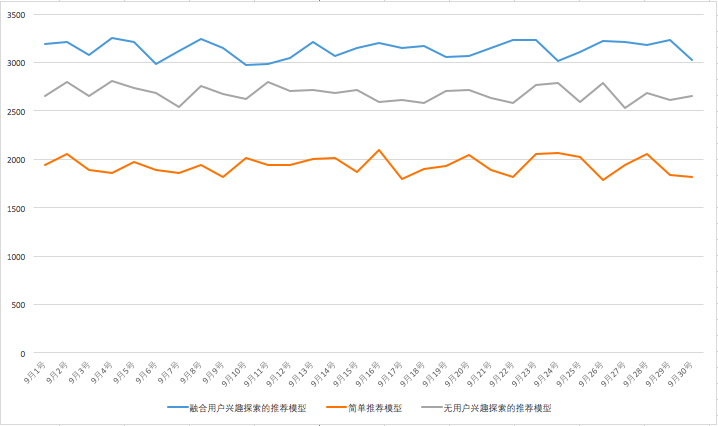
\includegraphics[scale=0.55]{figures/hl_themeNumber}}
    \figcaption{推荐多样性实验对比图}
    \label{pic:hl_themeNumber}
  \end{figure}

  我们对比了无兴趣探索模块的推荐模型、推荐热门商品的简单推荐模型和融合了兴趣探索模块的推荐模型在实验期间的点击购买转化率。\autoref{pic:hl_buyLookRatio}展示了不同模型的实验结果。图中,横坐标是时间变量,单位为天,纵坐标是点击购买转化率,每一条曲线代表了一个模型的点击购买转化率随时间变化的曲线。实验结果显示,融合了兴趣探索模块的推荐模型相对其他模型有更高的点击购买转化率。融合了兴趣探索模块的推荐模型的平均点击购买转化率是32.74\%,比推荐热门商品的简单推荐模型的平均点击购买转化率9.63\%高了23.11个百分点,相对于无兴趣探索模块的推荐模型的平均点击购买转化率17.54\%高了15.2个百分点。由此可见用户兴趣探索能够很好的提升点击购买转化率。
  \begin{figure}
  \centering
    \framebox{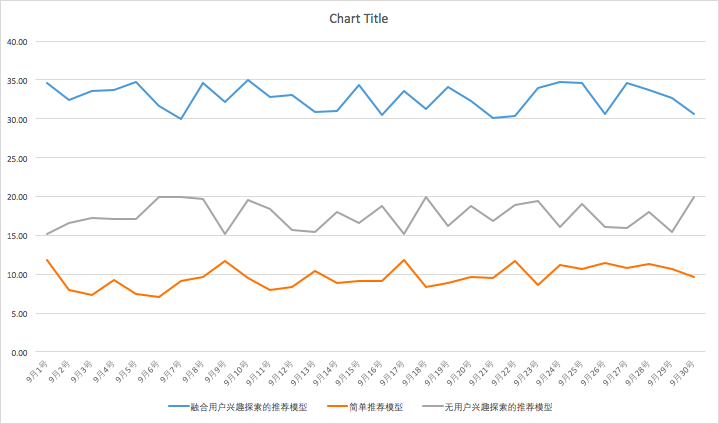
\includegraphics[scale=0.55]{figures/hl_buyLookRatio}}
    \figcaption{转化率实验对比图}
    \label{pic:hl_buyLookRatio}
  \end{figure}

\section{本章小结}
这一章主要研究了标签动态变化对推荐系统的影响,实际中用户同时会受到社会因素和个人因素的影响,但这两种因素在会产生不同强度的影响。在快速变化的系统中,用户行为更加会受到社会因素的影响,而在变化相对较慢的系统中,用户行为则更加受到个人因素的影响。本章首先介绍了用户行为数据的存储格式以及基于此的用户行为数据的的预处理。然后介绍了用户兴趣探索模块的组成内容,包括兴趣标签探测功能模块、长尾标签抽取功能模块和用户满意度量化功能模块,然后介绍了用户画像和用户兴趣探索的融合,最后给出了用户兴趣探索实验结果。
  
\chapter{结束语}
  如果说过去的五年是推荐系统大行其道的时间,那么个性化将成为推荐技术未来五年中最重要的革新之一。一个好的推荐系统需要满足的目标有:能实时提供个性推荐服务,推荐结果满足新颖性、惊喜性和长尾性,而且推荐结果必须足够及时,这样才能在用户浏览之后、购买之前就获得推荐服务,笔者通过引入用户画像模块和用户兴趣探索模块来达到以上目标。

  本文介绍的推荐系统由三部分模块组成:用户画像模块,用户兴趣探索模块、推荐算法模块。用户画像模块记录了用户长期的信息,刻画用户的基础类型。用户兴趣探索模块负责记录能够体现用户喜好的行为,比如购买、下载、评分等,这部分看起来简单,其实需要非常仔细的设计,比如说购买和评分这两种行为表达潜在的喜好程度就不尽相同。完善的行为记录需要能够综合多种不同的用户行为,处理不同行为的累加。推荐算法模块的功能则实现了对用户行为记录的分析、计算和排序。

  推荐系统的主要方法是通过分析用户的过去预测未来,因此基于用户画像模型的研究是一个很好的突破口,因为用户画像天然支持用户历史信息的存储、查询,同时对用户兴趣探索的研究,无论是从促进用户画像模型的角度出发,还是从实际需求来看,都具有重要的意义,本文的研究工作正是在这一背景下展开。

  \section{研究工作总结}
    本文对推荐系统特别是与用户画像相关的动态推荐系统的相关工作做了总结和回顾之外,主要的工作包括以下几个方面:
    \begin{itemize}
      \item 设计了用户画像模型:通过对基础静态数据、基础行为数据类型和高维数据类型进行建模,得出较为完整、准确的兴趣标签,解决新用户的冷启动问题,提升了推荐系统的精度。
      \item 设计了用户兴趣探索模型:通过量化用户满意度和计算用户和商品的相关度,实现了用户小众兴趣的探索功能,提升了推荐系统的动态推荐效果。
      \item 利用线性衰减算法成功融合用户长期兴趣和短期兴趣:本文在研究用户画像建模和用户兴趣探索的基础上,结合电子商务用户兴趣偏好变化频繁的特点,提出了基于线性衰减的用户兴趣融合模型。标签权重的线性衰减算法结合了手机主题用户长期兴趣和短期兴趣,能准确反映用户兴趣的变化趋势。
    \end{itemize}

  \section{对未来工作的展望}
  本文对推荐系统的用户画像和用户兴趣探索模型进行了较深入的研究,但是针对用户兴趣变化的推荐模型的实现还有很多工作要做。本人认为有待解决的问题有:
    \begin{itemize}
      \item 用户行为的离线和在线计算的分配:用户行为每天产生的数据量很大,哪些行为需要在线实时计算反馈,哪些行为只需要离线计算即可,需要根据具体业务的特点和用户习惯赋予每种行为一个权重,然后根据权重排名决定计算方式。因此,用户行为的特征提取、分析将是我们将来工作的一个重要方面。
      \item 用户兴趣探索模型对推荐系统的影响:本文的所有工作的评估集中在点击购买转换率上。但点击购买转换率并不是推荐系统追求的唯一指标,比如,预测用户可能会去看,从而给用户推荐热门商品,这并不是一个好的推荐。因为热门商品本身的转化率就很高,这里涉及到了推荐系统的长尾性,即用户希望推荐系统能够给他们新颖的推荐结果,而不是那些他们已经知道的物品。此外,推荐系统还有多样性等指标。如何利用时间信息,在不牺牲转换率的同时, 提高推荐的其他指标,是笔者将来工作研究的一个重要方面。
      \item 推荐系统随时间的进化:用户的行为和兴趣是随时间变化的,意味着推荐系统本身也是一个不断演化的系统。其各项指标,包括长尾度、多样性和点击率都是随着数据的变化而演化。如何让推荐系统能够通过利用实时变化的用户反馈,向更好的方面发展是推荐系统研究的一个重要方面。
    \end{itemize}

  最后,希望本文的研究工作能够对动态推荐系统的发展作出一定的贡献,并真诚的希望老师们提出宝贵的批评意见和建议。

%%%%%%%%%%%%%%%%%%%%%%%%%%%%%%
%% 附件部分
%%%%%%%%%%%%%%%%%%%%%%%%%%%%%%
\backmatter

  % 参考文献
  % 使用 BibTeX
  % 选择参考文献的排版格式。注意ustcbib这个格式不保证完全符合要求,请自行决定是否使用
  %\bibliographystyle{plain}%{GBT7714-2005NLang-UTF8}
  %\bibliography{bib/tex}
  %\nocite{*} % for every item
  % 不使用 BibTeX
  %\renewcommand{\baselinestretch}{0.5}
\begin{thebibliography}{10}

\bibitem{recmd-youtube}
Shumeet Baluja, Rohan Seth, D. Sivakumar, Yushi Jing, Jay Yagnik, Shankar Kumar, Deepak Ravichandran, and Mohamed Aly.2008.
\newblock {\em Video sug- gestion and discovery for youtube: taking random walks through the view graph}.
\newblock In Proceeding of the 17th international conference on World Wide Web, WWW ’08, pages 895–904.

\bibitem{recmd-system}
Francesco Ricci and Lior Rokach and Bracha Shapira.2011.
\newblock {\em Introduction to Recommender Systems Handbook[M]}.
\newblock Springer, 1-35. 

\bibitem{recmd-netflix}
Robert M. Bell and Yehuda Koren. December 2007.
\newblock {\em Lessons from the netflix prize challenge}.
\newblock SIGKDD Explor. Newsl., 9:75–79.

\bibitem{demo-data}
Bruce Krulwich.1997.
\newblock {\em Lifestyle finder: Intelligent user profiling using large-scale demographic data[C]}.
\newblock AI Magazine, 18(2):37–45.

\bibitem{cognitive-science}
Elaine Rich.1998.
\newblock {\em Readings in intelligent user interfaces[C]}.
\newblock chapter User modeling via stereotypes, 329–342. 

\bibitem{Forecast-principle}
J. Scott Armstrong, editor.2001.
\newblock {\em Principles of Forecasting - A Handbook for Researchers and Practitioners[M]}.
\newblock Kluwer Academic.

\bibitem{cf-sn}
Henry Kautz, Bart Selman, and Mehul Shah. March 1997.
\newblock {\em Referral web: combining social networks and collaborative filtering[C]}.
\newblock Commun. ACM, 40:63–65.

\bibitem{Amazon-cf}
Greg Linden, Brent Smith, and Jeremy York. January 2003.
\newblock {\em Amazon.com recommendation- s: Item-to-item collaborative filtering[C]}.
\newblock IEEE Internet Computing, 7:76–80.

\bibitem{info-overload}
Anne-F. Rutkowski and Carol S. Saunders.June 2010.
\newblock {\em Growing pains with information overload[C]}.
\newblock Computer, 43:96–95.

\bibitem{info-overload:1}
Anne-F. Rutkowski and Carol S. Saunders.June 2010.
\newblock {\em Growing pains with information overload[C]}.
\newblock Computer, 43:96–95.

\bibitem{recmd-history}
Liu, Yu; Li, Weijia; Yao, Yuan; Fang, Jing; Ma, Ruixin; Yan, Zhaofa.
\newblock {\em An Infrastructure for Personalized Service System Based on Web2.0 and Data Mining}.
\newblock International Conference on Intelligent Computing and Information Science. JAN 08-09, 2011.

\bibitem{user-interest}
Sia K.C, Zhu S.Chi, Hino Tseng, B.L.2006.
\newblock {\em Capturing User Interests by Both Exploitation and Exploration[C]}.
\newblock Technical report, NEC Labs America. 

\bibitem{recmd-xiangliang}
项亮. 2012.
\newblock {\em 推荐系统实践}.
\newblock 图灵原创,人民邮电出版社, 36:5–21.

\bibitem{content-based}
K Yoshii.2006.
\newblock {\em Hybrid Collaborative and Content-Based Music Recommendation Using Probabilistic Model with Latent User Preferences [C]}.
\newblock In: Proceedings of the International Conference on Music Information Retrieval.

\bibitem{collab-filter}
Jonathan L. Herlocker, Joseph A. Konstan, Loren G. Terveen, and John T. Riedl.January 2004.
\newblock {\em Evaluating collaborative filtering recommender systems[C]}.
\newblock ACM Trans.Inf.Syst, 22:5–53.

\bibitem{social-filter}
Henry Kautz, Bart Selman, and Mehul Shah.March 1997.
\newblock {\em Referral web: combining social networks and collaborative filtering[C]}.
\newblock Commun. ACM, 40:63–65.

\bibitem{cold-start}
Andrew I.Schein, Alexandrin Popescul, Lyle H.Ungar, David M.Pennock. 2002.
\newblock {\em Methods and Metrics for Cold-Start Recommendations[C]}.
\newblock New York City, New York: ACM. 253–260.

\bibitem{latent-cf}
Thomas Hofmann and Jan Puzicha.1999. 
\newblock {\em Latent class models for collaborative filtering[J]}.
\newblock In Proceedings of the Sixteenth International Joint Conference on Artificial Intelligence, IJCAI ’99,San Francisco, CA, USA, Morgan Kaufmann Publishers Inc, pages 688–693, 

\bibitem{date-mining}
Han Jiawei, Kamber, Micheline.2001.
\newblock {\em Data mining: concepts and techniques[C]}.
\newblock Morgan Kaufmann. 5.

\bibitem{info-retrieval}
Jansen B.J and Rieh S.2010.
\newblock {\em The Seventeen Theoretical Constructs of Information Searching and Information Retrieval[J]}.
\newblock Journal of the American Society for Information Sciences and Technology. 61(8)

\bibitem{long-tail}
O Celma. 2010.
\newblock{\em Music Recommendation and Discovery in the Long Tail[C]}.
\newblock Springer. 

\bibitem{temporal-cf}
Yehuda Koren.2009.
\newblock {\em Collaborative filtering with temporal dynamics[J]}.
\newblock In Proceedings of the 15th ACM SIGKDD international conference on Knowledge discovery and data mining, KDD ’09,New York, NY, USA., pages 447–456.

\bibitem{recmd-kmeans}
Hartigan, J.A.Wong, M.A.Algorithm.
\newblock {\em A k-Means Clustering Algorithm}.
\newblock Journal of the Royal Statistical Society, Series C. 1979, 28 (1): 100–108.

\bibitem{recmd-slopone}
Daniel Lemire, Anna Maclachlan.
\newblock {\em Slope One Predictors for Online Rating-Based Collaborative Filtering}.
\newblock In SIAM Data Mining (SDM'05), Newport Beach, California, April 21-23, 2005.

\bibitem{ab-test}
Kohavi, Ron, Longbotham, Roger.2015.
\newblock {\em Online Controlled Experiments and A/B Tests[C]}.
\newblock In Sammut.



\bibitem{recmd-Hybrid}
Robin Burke. November 2002.
\newblock {\em Hybrid recommender systems: Survey and experiments}.
\newblock User Modeling and User-Adapted Interaction, 12:331–370.

\bibitem{Personalization1}
Gediminas Adomavicius and Alexander Tuzhilin. 1999.
\newblock {\em User Profiling in Personalization Applications through Rule Discovery and Validation}.
\newblock ACM, 377-381.

\bibitem{Personalization2}
lbrahim Cingil, Asuman Dogac and Ayca Azgin.2000.
\newblock {\em A broader approach to personalization}.
\newblock mmunications of the ACM, 43(8): 136-141.

\bibitem{Personalization3}
Joseph Kramer, Sunil Noronha and John Vergo.2000.
\newblock {\em A user-centered design approach to personalization}.
\newblock Communications of the ACM, 43(8)44-48.

\bibitem{Personalization4}
Bamshad Mobasher, Honghua Dai, Tao Luo, Yuqing Sun and Jiang Zhu.2000.
\newblock {\em Integrating Web Usage and Content Mining for More Effective Personalization}.
\newblock Electronic Commerce and Web Technologies, 1875: 165-176.

\bibitem{Personalization5}
Bamshad Mobasher, Robert Cooley and Jaideep Srivastava.2000.
\newblock {\em Automatic personalization based on Web usage mining}.
\newblock Communications of the ACM, 43(8): 142-151.

\bibitem{Personalization6}
P. Chen, H. Xie, S. Maslov, and S. Redner.2007.
\newblock {\em Finding Scientific Gems with Google's PageRank Algorithm}.
\newblock Journal of Informetrics, 1(1):8--15.

\bibitem{Personalization7}
C. Basu, H. Hirsh, and W. Cohen.1998.
\newblock {\em Recommendation as Classification: Using Social and Content-Based Information in Recommendation}.
\newblock In Proc. of the 15th National Conference on Artificial Intelligence (AAAI ’98), 714–720.

\bibitem{Personalization8}
J. Teevan and S. T. Dumais and E. Horvitz.2005.
\newblock {\em Personalizing Search via Automated Analysis of Interests and Activities}.
\newblock . In Proc. of the 28th Annual International ACM SIGIR Conference on Research and Development in Information Retrieval (SIGIR 2005), 449–456,

\bibitem{Personalization9}
S. M. McNee, I. Albert, D. Cosley, S. L. P. Gopalkrishnan, A. M.Rashid, J. S. Konstan, and J. Riedl.2002.
\newblock {\em Predicting User Interests from Contextual Information}.
\newblock  In Proc. of the 2002 ACM Conference on Computer Supported Cooperative Work (CSCW ’02), 116–125,
\end{thebibliography}


  % 附录,没有请注释掉
  %\begin{appendix}
  %  
\chapter{中国科学技术大学研究生学位论文撰写规范}
\label{chap:requires}
\section*{以下文字仅作示例,一切以学校规定为准!}
研究生院规定在此下载\url{http://gradschool.ustc.edu.cn/ylb/material/xw/wdxz/1.doc}

研究生学位论文集中反映研究生在研究工作中所取得的成果,代表研究生研究工作的水平,也是申请和授予相应学位的主要依据。为提高研究生学位论文的撰写质量,做到学位论文在内容和格式上的规范化,我们编写了《中国科学技术大学研究生学位论文撰写规范》,供申请学位的研究生参考执行。其中参考文献著录规则我们根据GB/T 7714-2005的标准撰写。硕士和博士学位论文除在研究深度等方面要求不同外,撰写要求基本一致。

\section{内容要求}

\subsection{封面} 
采用研究生院规定的统一封面,封面包含内容如下: 
\subsubsection{密级} 涉密论文必须在论文封面标注密级(内部、秘密、机密),同时注明保密年限。
\subsubsection{论文题目} 应准确概括整个论文的核心内容,简明扼要,最多不超过30字,必要时可以加副标题。
\subsubsection{作者姓名} 英文封面中按英文习惯书写,即名在前。姓名需写全拼。
\subsubsection{学科专业} 写所在专业的全称,不可用简写。
\subsubsection{导师姓名} 一般允许有两名指导教师,主要指导教师姓名写在第一位,后附其职称,次要指导教师排第二位,也需注明职称。
\subsubsection{完成时间} 填写论文打印成文的年月日。

\subsection{中国科学技术大学学位论文原创性和授权使用声明}
本部分内容使用统一的模版,具体内容见格式范例,提交时作者须亲笔签名。

\subsection{摘要和关键词}
\subsubsection{中文摘要}
摘要是论文内容的总结概括,应简要说明论文的研究目的、基本研究内容、研究方法、创新性成果及其理论与实际意义,突出论文的创新之处。不宜使用公式、图表,不标注引用文献。 
\subsubsection{中文关键词} 
关键词是为了文献标引工作从论文中选取出来用以表示全文主题内容信息的单词和术语,一般3--8个词,要求能够准确概括论文的核心内容。
\subsubsection{英文摘要与关键词}
以中文书写的论文,内容与中文摘要和关键词完全一致,其他语种书写的论文以简略为原则,不需要相同。

\subsection{目录}
目录页由论文的章、条、附录等序号、名称和页码组成。论文中如图表较多,可以分别列出清单置于目次页之后。图的清单应有序号、图题和页码。表的清单应有序号、表题和页码。

\subsection{符号说明}
如果论文中使用了大量的物理量符号、标志、缩略词、专门计量单位、自定义名词和术语等,应编写成注释说明汇集表。若上述符号等使用数量不多,可以不设此部分,但必须在论文中出现时加以说明。

\subsection{正文}
正文是学位论文的主体,包括绪论、论文主体及结论等部分。
\subsubsection{绪论}
内容应包括:选题的背景和意义,文献综述及研究现状,研究内容与预期结果,研究方法和实验设计,论文结构安排等。要求实事求是,不夸大、缩小前人的工作和自己的工作,言简意赅,突出重点,不与摘要雷同。
\subsubsection{论文主体}
论文主体是正文的核心部分,占主要篇幅,它是将学习、研究和调查过程中筛选、观察和测试所获得的材料,经过加工整理和分析研究,由材料而形成论点。由于各学科及具体选题的差异,此部分不作统一规定。但总体内容必须实事求是,客观真切,准确完备,合乎逻辑,层次分明,简练可读。
\subsubsection{结论}
结论是对整个论文主要成果的总结,应明确、精炼、完整、准确。其中应明确指出本研究的创新点,对论文的学术价值和应用价值等加以预测和评价,说明研究中尚难解决的问题并提出今后进一步在本研究方向进行研究工作的设想或建议。

\subsection{参考文献}
本着以严谨求实的科学态度撰写论文,凡学位论文中有引用或参考、借用他人成果之处,均应详细列出所引文献的名称、作者、发表刊物、发表时间、卷号、页码等,严禁抄袭剽窃。  
\subsection{附录}
主要列入正文内过分冗长的公式推导,供查读方便所需的辅助性数学工具或表格,重复性数据图表,论文使用的缩写,程序全文及说明等。

\subsection{致谢}
对给予各类资助、指导和协助完成研究工作以及提供各种对论文工作有利条件的单位及个人表示感谢。致谢应实事求是,切忌浮夸与庸俗之词。

\subsection{在读期间发表的学术论文与取得的其他研究成果}
按学术论文发表的时间顺序,列齐本人在攻读学位期间发表或已录用的学术论文清单(发表刊物名称、卷册号、页码、年月及论文署名、作者排序)。其他研究成果可以是申请的专利、获得的奖项及完成的项目等。
 
\section{书写规定}

\subsection{论文的字数要求}
硕士学位论文要求不少于3万字,博士学位论文要求不少于5万字。

\subsection{文字、标点符号和数字}
除留学生和外语专业研究生外,学位论文一律用汉字书写。除非特殊需要,不得使用已废除的繁体字、异体字等不规范汉字。标点符号的用法以GB/T 15834—1995《标点符号用法》为准。数字用法以GB/T 15835—1995《出版物上数字用法的规定》为准。

留学生的学位论文所采用语种可以和导师商定,但论文封面须用中文。

\subsection{封面与扉页}
\subsubsection{秘级} 封面的秘级可以标注为内部、秘密和机密,各密级的保密时限分别为小于等于5年、小于等于10年和小于等于20年,非保密论文不标注密级。
\subsubsection{题目} 题目中避免使用缩略词、首字母缩写字、字符、代号和公式等。
\subsubsection{日期} 封面的日期用汉字书写。
\subsubsection{扉页} 扉页的内容与封面一致。扉页后,需给出英文的封面。其他语种书写的论文还需在英文封面后附上正文所用语种书写的封面。

\subsection{目录}
目录应包括论文的全部内容,包括中英文摘要和附录等,正文章节题名要求编到第3级标题,即×.×.×。一级标题顶格书写,二级标题缩进一个汉字符位置,三级标题缩进两个汉字符位置。

\subsection{摘要与关键词}
\subsubsection{摘要}
摘要分中文和英文两种,中文在前,英文在后。标题摘要二字中间空一格。摘要的字数,硕士学位论文建议1000字以内,博士学位论文建议3000字以内。留学生用其他语种撰写学位论文时,中文摘要应不少于6000汉字。摘要中不得出现图片、图表、表格或其他插图材料。英文摘要与中文摘要应完全一致。
\subsubsection{关键词}
关键词以显著的字符另起一行并隔行排列于摘要下方,左顶格。中文关键词间空一格,英文关键词间用逗号隔开。

\subsection{论文正文}
\subsubsection{章节及各章标题}
论文正文分章节撰写,每章应另起一页。

各章标题字数一般应在15字以内,不使用标点符号。标题中尽量不采用英文缩写词,对必须采用者,应使用本行业的通用缩写词。
\subsubsection{序号}
\paragraph{标题序号}
论文标题分层设序。层次以少为宜,根据实际需要选择。各层次标题一律用阿拉伯数字连续编号;不同层次的数字之间用小圆点“.”相隔,末位数字后面不加点号,如“1”,“1.1”,“1.1.1”等;各层次的序号均左起顶格排,后空1个字距接排标题。例如:

第1章 ××××(大标题) 

1.1 ××××(一级节标题)

1.1.1 ××××(二级节标题)

1.1.1.1 ××××(根据需要,也可设三级节标题)

第2章 ××××(大标题)

2.1 ××××(一级节标题)

2.1.1 ××××(二级节标题)

\paragraph{图表等编号} 
论文中的图、表、附注、公式、算式等,一律用阿拉伯数字分章依序连续编码。其标注形式应便于互相区别,如:图 l.1(第1章第一个图)、图2.2(第二章第二个图);表3.2(第三章第二个表)等。
\paragraph{页码}
页码从绪论开始按阿拉伯数字(1,2,3……)连续编排,此前的部分(中英文摘要、目录等)用大写罗马数字(I,II,III…)单独编排,页码位置居于页脚居中。封面、扉页、创新性声明等不编页码。
\subsubsection{页眉}
页眉从中文摘要开始,内容与该部分的一级标题相同,奇偶页相同,各部分的首页也需有页眉。
\subsubsection{名词和术语}
科技名词术语及设备、元件的名称,应采用国家标准或部颁标准中规定的术语或名称。标准中未规定的术语要采用行业通用术语或名称。全文名词术语必须统一。一些特殊名词或新名词应在适当位置加以说明或注解。

采用英语缩写词时,除本行业广泛应用的通用缩写词外,文中第一次出现的缩写词应该用括号注明英文原词。
\subsubsection{量和单位}
量和单位要严格执行GB 3100~3102-93(国家技术监督局1993-12-27发布,1994-07-01实施)有关量和单位的规定。

量的符号一般为单个拉丁字母或希腊字母,并一律采用斜体(pH例外)。为区别不同情况,可在量符号上附加角标。 

在表达量值时,在公式、图、表和文字叙述中,一律使用单位的国际符号,且无例外地用正体。单位符号与数值间要留适当间隙。具体可参见下列表达式3.1。

\subsubsection{图和表}
\paragraph{图}
图应具有“自明性”,即只看图、图题和图例,不阅读正文,就可理解图意。每一图应有简短确切的题名,连同图号置于图下。

图的位置在相关说明文字之后,随文排。坐标比例不宜过大,同一图上不同曲线的点要分别用不同形状的标识符标出。图中的术语、符号、单位等应与正文表述中所用一致。

图题应简明。图号和图题间空1个字符位置,居中排于图的下方。

必要时,应将图上的符号、标记、代码,以及实验条件等,用最简练的文字,横排于图题下方,作为图例说明(图注)。

\paragraph{表}
表的位置也在相应说明文字之后,随文排。表中参数应标明量和单位的符号。表应有自明性。每一表应有简短确切的题名,连同表号置于表上,表号与表题间空一个字符位置。表号用阿拉伯数字分章编号,如第3章第2个表的表号表示为“表3.2”。

表格太大需要转页时,需要在续表上方注明“续表”,表头也应重复排出。

必要时应将表中的符号、标记、代码,以及需要说明事项,以最简练的文字,横排于表题下,作为表注。相关要求同于图注。

\subsubsection{表达式}
表达式主要指数字表达式,也包括文字表达式。表达式需另行起排,原则上应居中,用阿拉伯数字分章编号。序号加圆括号,右顶格排。例如,第3章第1个表达式:

较长的式如必须转行,只能在+,-,×,÷,<,>处转行,序号编于最后一行的最右边。

\subsection{参考文献}
参考文献参照GB/T 7714-2005《文后参考文献著录规则》执行。推荐使用著者-出版年制,即在正文引用文献处标注著者姓名与出版年份,在文后的参考文献表中标注参考文献的详细信息。
\subsubsection{著者-出版年制在正文中的标注方式}

正文中的标注方式分两种:其一,正文里已出现著作者姓名的,在其后用圆括号附上出版年份即可;其二,正文里仅提及有关的资料内容而未提到著作者,则在相应文句处用圆括号标注著作者姓名和出版年份,两者之间加逗号。

例如:

Park et al(1995)根据Laurentia西缘放射状基性岩墙的研究以及与地幔柱有关的澳大利亚Gairdner岩墙群的研究,首次提出约780Ma地幔柱导致Rodinia超大陆的裂解。

其中关于成冰系顶底界时限和冰川活动年龄、超大陆裂解的起始时间和持续时间……是当前中国地球科学界十分活跃并得到迅速发展的研究领域(王平,2003)。

引用同一著者在同一年份出版的多篇文献时,在出版年份之后用英文小写字母a、b、c……区别。如:(王平,2005a);(王平,2005b)

多处引用同一著者的同一文献时,在“()”外以角标的形式著录引文页码。引用有两个以上同姓的著者的外文文献时,则著者要加名字的缩写,但不必加缩写点。

引用多位著者的文献时,对欧美著者只需标注第一个著者的姓,其后附“et al”,仅两位作者的也可全部注出,中间用“and”;对中国著者应该标注第一著者的姓名,其后附“等”字,姓名与“等”字之间留1个空格。例如:……(王平 等,2005) ……。

同一处引用多篇文献时,按出版年份由近及远依次标注,中间用逗号分开。

\subsubsection{著者-出版年制参考文献表的编排}
 参考文献表加居中标题——“参考文献”,并列入全书目录。

凡正文里括注了著者姓名和年份的,其文献都必须列入参考文献表。

参考文献表中的条目(不排序号),先按语种分类排列,语种顺序是:中文、日文、英文、俄文、其他文种。然后,中文和日文按第一著者的姓氏笔画排序,中文也可按汉语拼音字母顺序排列,西文和俄文按第一著者姓氏首字母顺序排列。

在参考文献中,当一个著者有多篇文献并为第一著作者时,他单独署名的文献排在前面(并按出版年份的先后排列),接着排他与其他人合写的文献。

著录项目与GB/T 7714-2005《文后参考文献著录规则》中规定的顺序编码制基本相同,不同的仅为出版年份排于编著者之后。
\subsubsection{参考文献标注的注意事项}
编著者姓名,一律姓在前、名字在后。西文和俄文的姓全部著录,名字可用大写首字母(不加缩写点);如果姓和名的首字母相同,便要用全名。

以机构和团体署名的文献,此机构或团体可作为编著者,但要用全称,而不用简称或缩写。

编著者不明的文献,编著者一项应注明“佚名”,或用其他与之相应的词。 

编著者为3人以下时全部著录,用逗号分隔,3人以上可只著录前3人,后加“,等”,外文用“,et al”,“et al”不必用斜体。

外文文献大写字母的使用要符合文种本身的习惯用法。

外文期刊刊名可列出全名,也可列惯用缩写刊名(缩写点可加,也可不加,但全文要统一)。只有一个词的刊名不能缩写。期刊名排正体。

期刊只列出卷号,不必标“卷”或“Vol”等;如果是分卷图书,则应加“卷”或“册”或“Vol”或其他语种相应的词(外文缩写词不加缩写点,首字母大小写应全文统一)。

参考文献的版次、卷、期、页码等数字一律用阿拉伯数字表示。版次中中文版次著录为“第2版”、“第3版”……(第1版不必列出),西文文献的版次著录为“2nd ed”、“3rd ed”或其他语种相应的词 。

出版年采用公元纪年,并用阿拉伯数字著录。如有其他纪年形式时,将原有的纪年形式置于“( )”内。

如:1947(民国三十六年)

日文文献中的汉字要用日文汉字。

参考文献中使用的标点符号:

,用于多著者姓名之间,出版者和年或卷(期)之间,期刊名和年或卷之间,“等”或“译”字、专利号等之前。

:用于副题名之前、出版地之后,或引文页码、析出文献页码、专利国别前。

()用于期号、报纸的版次、电子文献更新或修改日期以及非公元纪年。

[] 用于序号、文献类型、电子文献的引用日期以及自拟的的信息。

∥用于专著中的析出文献的出处项前。

- 用于起讫序号和起讫页码间。

. 用于其余各项目之后。

\subsubsection{顺序编码制的著录规则}
参考文献如果按照顺序编码制著录,可参照GB/T 7714-2005《文后参考文献著录规则》执行。


\section{排版和印刷要求}略

\chapter{关于规范本科毕业论文(设计)格式和统一封面的通知}
\section*{以下文字仅作示例,一切以学校规定为准!}
教务处规定在此下载\url{http://202.38.70.92/bklw.doc}

\hspace{-2em}各院系:

鉴于目前各院系本科毕业论文(设计)存在着论文格式不够规范、封面不统一的状况,为加强本科毕业论文的管理,提高论文质量,同时规范全校本科毕业论文(设计)格式,现对本科毕业论文格式和统一封面规定如下:
\begin{enumerate}
\item 本科毕业论文按编排顺序应包括以下内容:封面、扉页、致谢、目录、中文内容摘要、英文内容摘要、正文章节、参考文献或资料注释、附录等。
\item 本科毕业论文的格式要求:
\begin{enumerate}
\item 封面中“论文题目”等内容用四号宋体。
\item 除封面、扉页外,每面上部加页眉,用小5号字标注“中国科学技术大学本科毕业论文”,居中。
\item 从目录页开始在每面底部居中用小五宋体连续编页码。
\item 论文的“致谢”、“目录”等标题用小二号黑体字,居中。
\item 目录一般列三级,后附规范的页号。
\item 正文中的标题分章、节、段三级;章、节标题居中,段标题居左,分别用三号黑体、小三黑体、四号黑体。
\item 具体内容用小四号宋体,每行间距为22磅,科学公式和符号要符合国标,公式要单独占行、居中、行距为单倍行距。
\item 表格、插图全文要分别统一编号或按章编号,标题用小四宋体:(表格标题居表上方,插图标题居图下方),居中。
\item 参考文献的内容包括:序号、作者名、书名或文章名、刊物名或出版社名、
刊物期卷、页和日期,用小四宋体,外文期刊名用白斜体。
\item 附录为:
\begin{enumerate}
\item 重要参考文献中相关内容和章节复印件;
\item 作者或导师所做的与本论文有关的成果复印件。
要求用A4纸复印附于参考文献后。
\end{enumerate}
\end{enumerate}
\item 本科毕业论文(设计)封面学校已统一印制,请到教材科领购。
\item 装订要求:每份论文必须用A4纸打印(复印)、装订成册(教材科可提供复印、装订业务)。另外,校级优秀毕业论文必须提交一份线装毕业论文交档案馆收藏。
\item 具体格式详见附件式样。
\end{enumerate}
\begin{flushright}
中国科技大学教务处

二OO二年三月二十八日
\end{flushright}
附件:本科毕业论文(设计)式样

(略)

  %\end{appendix}

  \makeatletter
  \ifustc@bachelor\relax\else
    % 致谢
	
\begin{thanks}

人生就是一个关于成长的漫长故事。而在中科大求学作为本人人生体验的一部分,亦是这样的一段故事。在此的俩年半,俯仰之间,科大的“问道”、“学术”于此,让我经历了这样的三段成长:学于师友,安于爱好,观于内心。

“古之学者必有师,师者,所以传道、授业、解惑也”。师友的教诲不可能一直跟着自己,可是他们治学态度却融入了我的人生观。授课的华保健老师的严谨、郭燕老师的认真、丁菁老师的直率、席菁老师的踏实都曾触动我,并给予我前进方向上的指引。

本论文内容为数据挖掘在电商行业的工程实现,因此有一段真实的、贴近数据挖掘领域的实习经历尤为重要。感谢我在苏州国云数据公司实习的 CEO 马晓东学长,让我有机会一窥大数据行业的内幕;感谢我在小米实习的导师方流博士,感谢我在滴滴出行工作的机器学习研究院李佩博士,让我成为大数据挖掘工程师的梦想又更近了一步;感谢我的导师周武旸教授和张四海教授,指导我完成论文。
向师友和书籍学习,是从外界汲取;只有回归到自己的内心和思绪才能沉淀.在每个夜幕深沉或是晨曦初露的时刻里,感受自己情绪的流动,反思自己的取舍得失,然后才有了融于师友和书籍时的奋进。这样的三段成长,如今已是一体,不断地相互印证与反馈!

“逝者如斯夫,不舍昼夜”。成长亦复如是,不断的和昨日的自己告别。但是,一路有你,真好!相会是缘,同行是乐,共事是福!

\vskip 18pt

\begin{flushright}

~~~~\ustc@author~~~~

\today

\end{flushright}

\end{thanks}
%硕博致谢部分
    % 发表文章目录
    %\include{chapter/pub}
  \fi
  \makeatother

\end{document}
